% !TeX program = xelatex
% !TeX encoding = UTF-8
% Spedizione P08 · Collocare nel tempo il massimo di un proxy
% Presentazione della spedizione P08 nella serie planetaria di GeoStat Lab.
% Compilazione: xelatex -interaction=nonstopmode P08_Proxy.tex (due passaggi)
% 28 slide. Diagrammi TikZ, figure vettoriali da R/P08_figure.R, codice R, dati ed esperimenti inclusi.
\RequirePackage{fix-cm}
\documentclass[12pt,aspectratio=1610]{beamer}
\geometry{paperwidth=20cm,paperheight=12.5cm}
\usepackage[italian,provide=*]{babel}
\usepackage{fontspec,adjustbox,tabularx}
\IfFontExistsTF{NimbusSans-Regular.otf}{
\setsansfont{NimbusSans-Regular.otf}[BoldFont=NimbusSans-Bold.otf,ItalicFont=NimbusSans-Italic.otf,BoldItalicFont=NimbusSans-BoldItalic.otf]
\setmainfont{NimbusSans-Regular.otf}[BoldFont=NimbusSans-Bold.otf,ItalicFont=NimbusSans-Italic.otf,BoldItalicFont=NimbusSans-BoldItalic.otf]
}{
\setsansfont{TeX Gyre Heros}
\setmainfont{TeX Gyre Heros}
}
\IfFontExistsTF{DejaVu Sans Mono}{
\setmonofont{DejaVu Sans Mono}[Scale=.88]
}{\setmonofont{Latin Modern Mono}[Scale=.88]}
\usefonttheme{professionalfonts}
\usepackage{amsmath,amssymb,booktabs,array,graphicx,tikz,bookmark}
\usetikzlibrary{calc,positioning,arrows.meta}
\graphicspath{{Figure/}}
\definecolor{Paper}{HTML}{F8F6F1}
\definecolor{Ink}{HTML}{253344}
\definecolor{Navy}{HTML}{15283E}
\definecolor{Quantum}{HTML}{5146A5}
\definecolor{Classical}{HTML}{087C74}
\definecolor{Muted}{HTML}{657180}
\definecolor{Rule}{HTML}{D6DAD9}
\definecolor{Night}{HTML}{112236}
\definecolor{Lilac}{HTML}{ABB5FF}
\definecolor{Mint}{HTML}{72D8C8}
\setbeamercolor{background canvas}{bg=Paper}
\setbeamercolor{normal text}{fg=Ink}
\setbeamertemplate{navigation symbols}{}
\setbeamertemplate{headline}{}
\setbeamertemplate{footline}{}
\setbeamersize{text margin left=0pt,text margin right=0pt}
\hypersetup{colorlinks=true,linkcolor=Classical,urlcolor=Classical,pdfpagemode=UseOutlines,pdfstartview=Fit,
 pdftitle={Spedizione P08 · Collocare nel tempo il massimo di un proxy},pdfauthor={GeoStat Lab · materiali di Marzio De Corato},
 pdfsubject={GeoStat Lab · P08}}
\bookmarksetup{open,openlevel=0,depth=2}
\newsavebox{\BodyBox}
\newsavebox{\SideBox}
\newsavebox{\RecallBox}
\newsavebox{\TitleBox}
\newcommand{\MeasureBox}[2]{\typeout{REVIEWBOX:#1:\the\wd#2:\the\ht#2:\the\dp#2}}

% Revisione completa: diagrammi TikZ, formalismo e box R.
\usepackage[most]{tcolorbox}
\usepackage{listings}
\usetikzlibrary{fit,backgrounds,matrix,decorations.pathreplacing}
\definecolor{GeoA}{HTML}{1D7890}
\definecolor{GeoB}{HTML}{C57E42}
\definecolor{GeoC}{HTML}{7363AA}
\definecolor{GeoTint}{HTML}{F0F4F3}
\lstdefinestyle{GeoR}{language=R,basicstyle=\ttfamily\fontsize{9.2}{12.2}\selectfont,
 keywordstyle=\color{Quantum}\bfseries,commentstyle=\color{Classical},stringstyle=\color{GeoB},
 numbers=left,numberstyle=\tiny\color{Muted},numbersep=4pt,showstringspaces=false,
 columns=fullflexible,keepspaces=true,breaklines=true,xleftmargin=1.15em,
 frame=none,aboveskip=0pt,belowskip=0pt,tabsize=2}
\newsavebox{\PilotLeftBox}
\newsavebox{\PilotRightBox}
\newcommand{\PLabel}[1]{\par{\color{Classical}\bfseries\fontsize{9}{11}\selectfont\MakeUppercase{#1}}\par\vspace{1.8mm}}
\newcommand{\PBody}[1]{\par{\fontsize{11.3}{14.8}\selectfont #1\par}}
\newcommand{\PSmall}[1]{\par{\fontsize{9.8}{13.1}\selectfont #1\par}}
\newcommand{\PCode}[2]{%
\begin{tcolorbox}[enhanced,arc=1.8mm,boxrule=.65pt,
  colback=white,colframe=Classical!75!Navy,colbacktitle=Navy,
  coltitle=white,fonttitle=\bfseries\fontsize{9.6}{12}\selectfont,
  title={#1},left=1.7mm,right=1.3mm,top=1.5mm,bottom=1.3mm,
  before skip=1mm,after skip=1mm]
\lstinputlisting[style=GeoR]{Codice/#2}
\end{tcolorbox}}
\newcommand{\PInfo}[1]{%
\begin{tcolorbox}[enhanced,arc=1.6mm,boxrule=.55pt,colback=GeoTint,
 colframe=Rule!80!Classical,left=2.3mm,right=2.3mm,top=2mm,bottom=2mm,
 before skip=1mm,after skip=1mm]
\PSmall{#1}\end{tcolorbox}}
\tikzset{
 pFlow/.style={draw=Classical!45,fill=white,rounded corners=2mm,
  line width=.7pt,align=center,minimum height=1.1cm,font=\sffamily\fontsize{10}{12}\selectfont},
 pEdge/.style={-{Latex[length=2.3mm]},draw=Classical,line width=.95pt},
 pGroup/.style={draw=Rule,fill=white,rounded corners=2mm,line width=.65pt},
 pDotA/.style={circle,fill=GeoA,inner sep=1.25pt},
 pDotB/.style={circle,fill=GeoB,inner sep=1.25pt},
 pDotC/.style={circle,fill=GeoC,inner sep=1.25pt}
}
\newcommand{\PilotChrome}[4]{%
  \node[anchor=north west,inner sep=0,text width=17.7cm] at ([xshift=.95cm,yshift=-.55cm]current page.north west) {\color{Navy}\bfseries\fontsize{20.6}{24.5}\selectfont #1};
  \node[anchor=north east,inner sep=0] at ([xshift=19.05cm,yshift=-.14cm]current page.north west) {\color{Classical}\fontsize{8}{10}\selectfont\hyperlink{slide2}{#2}};
  \draw[Classical,line width=1.2pt] ([xshift=.95cm,yshift=-1.7cm]current page.north west)--([xshift=2.35cm,yshift=-1.7cm]current page.north west);
  \draw[Rule,line width=.65pt] ([xshift=.95cm,yshift=-10.36cm]current page.north west)--([xshift=19.05cm,yshift=-10.36cm]current page.north west);
  \node[anchor=north west,inner sep=0] at ([xshift=.96cm,yshift=-10.55cm]current page.north west) {\color{Classical}\bfseries\fontsize{9.1}{12}\selectfont DA RICORDARE};
  \node[anchor=north west,inner sep=0,text width=14.3cm] at ([xshift=4.2cm,yshift=-10.53cm]current page.north west) {\color{Ink}\fontsize{10.3}{13.8}\selectfont #4};
  \draw[Rule,line width=.35pt] ([xshift=.95cm,yshift=-11.92cm]current page.north west)--([xshift=19.05cm,yshift=-11.92cm]current page.north west);
  \node[anchor=north west,inner sep=0] at ([xshift=.95cm,yshift=-12.06cm]current page.north west) {\color{Muted}\fontsize{7.7}{9.2}\selectfont Spedizione P08 · Collocare nel tempo il massimo di un proxy};
  \node[anchor=north east,inner sep=0] at ([xshift=19.05cm,yshift=-12.06cm]current page.north west) {\color{Muted}\fontsize{7.7}{9.2}\selectfont #3/28};
}


% Stili comuni per i diagrammi scientifici della revisione completa.
\tikzset{
 pAxis/.style={-{Latex[length=2mm]},draw=Muted,line width=.65pt},
 pNote/.style={font=\sffamily\fontsize{9}{11.5}\selectfont,text=Muted,align=center},
 pLabel/.style={font=\sffamily\fontsize{10}{12.5}\selectfont,text=Ink,align=center}
}
\newsavebox{\FullWideBox}
\setlength{\emergencystretch}{1em}




\newcommand{\PLab}[2]{\par{\color{Classical}\bfseries\fontsize{9}{11}\selectfont
\href{#1}{\MakeUppercase{#2}}}\par\vspace{1.8mm}}

\definecolor{Measure}{HTML}{A05B10}\definecolor{Rose}{HTML}{9B4564}\definecolor{Wash}{HTML}{EAE7F6}\definecolor{Gold}{HTML}{EEC184}
\tikzset{arr/.style={-{Stealth[length=2mm]},line width=.8pt,draw=Classical}}
\newcommand{\Colonna}[2]{\begin{adjustbox}{max totalsize={#1}{7.95cm},valign=t}\begin{minipage}[t]{#1}\raggedright\fontsize{11.3}{14.8}\selectfont #2\end{minipage}\end{adjustbox}}
\begin{document}

\begin{frame}[plain]\hypertarget{slide1}{}\bookmark[level=0,page=1]{Spedizione P08}
\begin{tikzpicture}[remember picture,overlay]
\fill[Night](current page.south west) rectangle(current page.north east);
\IfFileExists{Scena/copertina.jpg}{\node[inner sep=0] at(current page.center){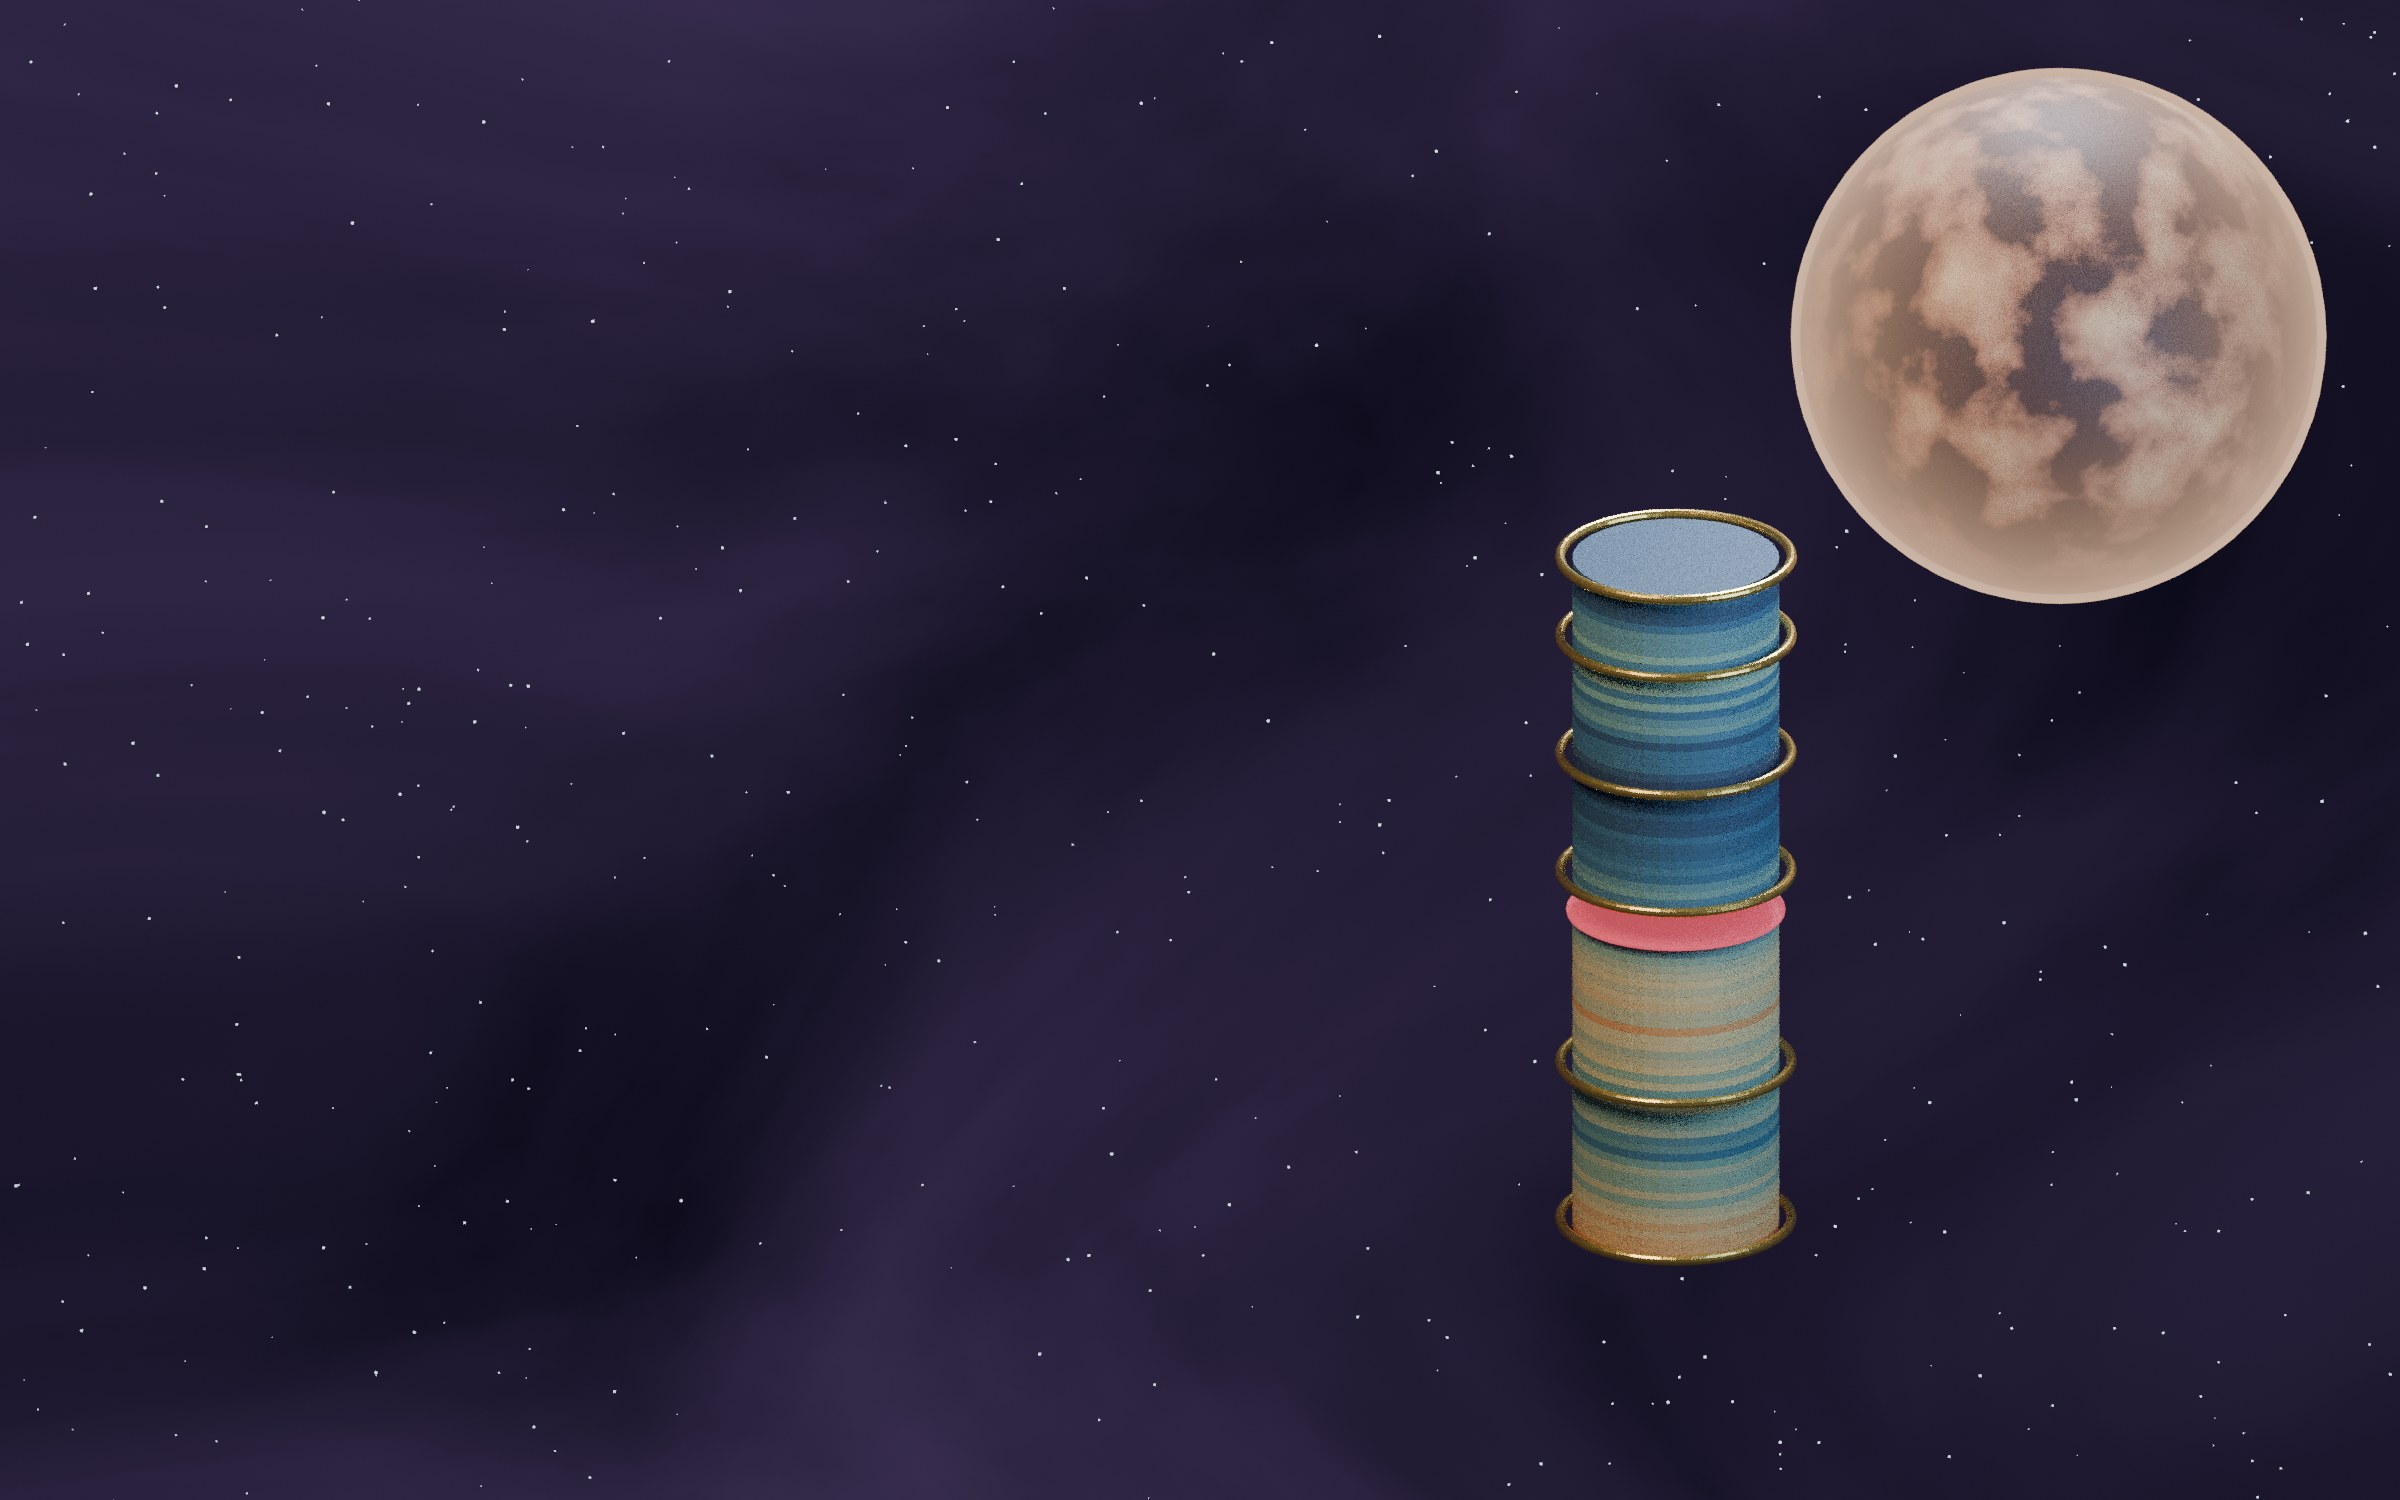
\includegraphics[width=20cm,height=12.5cm]{Scena/copertina.jpg}};}{}
\node[anchor=north west,inner sep=0] at([xshift=1.05cm,yshift=-1.10cm]current page.north west){\color{Mint}\bfseries\fontsize{23}{28}\selectfont SPEDIZIONE P08};
\node[anchor=north west,inner sep=0] at([xshift=1.07cm,yshift=-2.16cm]current page.north west){\color{white}\fontsize{9}{12}\selectfont MACROPROGETTO P08 · SCIENZE DELLA TERRA};
\draw[Mint,line width=1.5pt]([xshift=1.07cm,yshift=-2.78cm]current page.north west)--([xshift=2.6cm,yshift=-2.78cm]current page.north west);
\node[anchor=north west,inner sep=0] at([xshift=1.05cm,yshift=-3.35cm]current page.north west){\begin{minipage}{9.2cm}\raggedright\color{white}\bfseries\fontsize{28.5}{34.5}\selectfont Collocare nel tempo\\il massimo\\di un proxy\end{minipage}};
\node[anchor=north west,inner sep=0] at([xshift=1.07cm,yshift=-7.88cm]current page.north west){\begin{minipage}{8.9cm}\raggedright\color{Lilac}\fontsize{12.2}{17}\selectfont Sei ancore e ottantuno misure\end{minipage}};
\node[anchor=north west,inner sep=0] at([xshift=1.07cm,yshift=-8.70cm]current page.north west){\begin{minipage}{8.9cm}\raggedright\color{white!75}\fontsize{10.3}{14.5}\selectfont Ancore cronologiche, propagazione dell’incertezza e discontinuità sedimentarie\end{minipage}};
\node[anchor=north west,inner sep=0] at([xshift=1.07cm,yshift=-10.52cm]current page.north west){\color{white}\fontsize{10.5}{14}\selectfont GeoStat Lab · corso di Marzio De Corato};
\node[anchor=north west,inner sep=0] at([xshift=1.07cm,yshift=-11.17cm]current page.north west){\color{Mint}\fontsize{8.8}{11}\selectfont\href{https://creativecommons.org/licenses/by-nc-sa/4.0/}{Impaginazione da Tessera · CC BY-NC-SA 4.0}};
\end{tikzpicture}\end{frame}

\begin{frame}[plain]\hypertarget{slide2}{}
\bookmark[level=1,page=2]{Indice della presentazione}
\begin{tikzpicture}[remember picture,overlay]
\PilotChrome{Indice della presentazione}{PERCORSO}{2}{I titoli dell’indice aprono i capitoli. Il nome del capitolo in alto riporta a questa pagina.}
\node[anchor=north west,inner sep=0] at([xshift=.96cm,yshift=-2.12cm]current page.north west){\Colonna{9.40cm}{\PLabel{Capitoli}
{\fontsize{10.7}{13.5}\selectfont\hyperlink{slide4}{Ancore e interpolazione cronologica\hfill 4}\par}\vspace{.16cm}
{\fontsize{10.7}{13.5}\selectfont\hyperlink{slide9}{Scenari di incertezza cronologica\hfill 9}\par}\vspace{.16cm}
{\fontsize{10.7}{13.5}\selectfont\hyperlink{slide13}{Massimo osservato e interpretazione temporale\hfill 13}\par}\vspace{.16cm}
{\fontsize{10.7}{13.5}\selectfont\hyperlink{slide17}{Hiatus e conclusione condizionata\hfill 17}\par}\vspace{.16cm}
{\fontsize{10.7}{13.5}\selectfont\hyperlink{slide20}{Laboratori della spedizione\hfill 20}\par}\vspace{.16cm}

}};
\node[anchor=north west,inner sep=0] at([xshift=10.85cm,yshift=-2.12cm]current page.north west){\Colonna{8.16cm}{\PLabel{Percorso di lettura}
\PBody{Il percorso interpola le ancore, propaga l’incertezza cronologica con scenari perturbati, colloca il massimo osservato e discute l’effetto di una discontinuità. I laboratori finali riprendono le tre fasi della spedizione.}
\PInfo{Le pagine Scenario A e Confronto riprendono gli esperimenti nel browser con dati sintetici. I valori di partenza del simulatore differiscono da quelli del caso.}
\href{https://marzione00.github.io/Lab_Geo/\#modulo-P08}{\color{Classical}\bfseries Apri la spedizione P08 su GeoStat Lab}
}};
\end{tikzpicture}\end{frame}

\begin{frame}[plain]\hypertarget{slide3}{}
\bookmark[level=1,page=3]{A quale età corrisponde il massimo del proxy, e quanto dipende dalla cronologia adottata?}
\begin{tikzpicture}[remember picture,overlay]
\PilotChrome{{\fontsize{15.3}{19}\selectfont A quale età corrisponde il massimo del proxy, e quanto dipende dalla cronologia adottata?}}{IL CASO GUIDA}{3}{La copertina è una scena illustrativa: i dischi della carota seguono i valori del proxy, gli anelli dorati le ancore.}
\node[anchor=north west,inner sep=0] at([xshift=.96cm,yshift=-2.12cm]current page.north west){\Colonna{9.40cm}{{\centering\resizebox{0.97\linewidth}{!}{\begin{tikzpicture}[x=1cm,y=1cm,every node/.style={font=\sffamily\fontsize{10}{12}\selectfont,text=Ink}]
\draw[draw=Classical,fill=Classical!8,rounded corners=2mm,line width=.7pt] (0,0.00) rectangle (8.6,-0.78);
\node[circle,anchor=center,fill=Classical,inner sep=0,minimum size=.5cm,text=white,font=\sffamily\bfseries\fontsize{9}{10}\selectfont] at (.48,-0.39) {1};
\node[anchor=west,text width=7.4cm,align=left] at (.95,-0.39) {Ancore e interpolazione cronologica};
\draw[pEdge] (.48,-0.80)--(.48,-1.02);
\draw[draw=Classical,fill=Classical!8,rounded corners=2mm,line width=.7pt] (0,-1.04) rectangle (8.6,-1.82);
\node[circle,anchor=center,fill=Classical,inner sep=0,minimum size=.5cm,text=white,font=\sffamily\bfseries\fontsize{9}{10}\selectfont] at (.48,-1.43) {2};
\node[anchor=west,text width=7.4cm,align=left] at (.95,-1.43) {Scenari di incertezza cronologica};
\draw[pEdge] (.48,-1.84)--(.48,-2.06);
\draw[draw=Classical,fill=Classical!8,rounded corners=2mm,line width=.7pt] (0,-2.08) rectangle (8.6,-2.86);
\node[circle,anchor=center,fill=Classical,inner sep=0,minimum size=.5cm,text=white,font=\sffamily\bfseries\fontsize{9}{10}\selectfont] at (.48,-2.47) {3};
\node[anchor=west,text width=7.4cm,align=left] at (.95,-2.47) {Massimo osservato e interpretazione temporale};
\draw[pEdge] (.48,-2.88)--(.48,-3.10);
\draw[draw=Classical,fill=Classical!8,rounded corners=2mm,line width=.7pt] (0,-3.12) rectangle (8.6,-3.90);
\node[circle,anchor=center,fill=Classical,inner sep=0,minimum size=.5cm,text=white,font=\sffamily\bfseries\fontsize{9}{10}\selectfont] at (.48,-3.51) {4};
\node[anchor=west,text width=7.4cm,align=left] at (.95,-3.51) {Hiatus e conclusione condizionata};
\draw[pEdge] (.48,-3.92)--(.48,-4.14);
\draw[draw=GeoB,fill=GeoB!8,rounded corners=2mm,line width=.7pt] (0,-4.16) rectangle (8.6,-4.94);
\node[circle,anchor=center,fill=GeoB,inner sep=0,minimum size=.5cm,text=white,font=\sffamily\bfseries\fontsize{9}{10}\selectfont] at (.48,-4.55) {L};
\node[anchor=west,text width=7.4cm,align=left] at (.95,-4.55) {Laboratori della spedizione};
\end{tikzpicture}
}\par}
\PSmall{Capitoli della spedizione; L indica i laboratori conclusivi.}
}};
\node[anchor=north west,inner sep=0] at([xshift=10.85cm,yshift=-2.12cm]current page.north west){\Colonna{8.16cm}{\PLabel{Il caso}
\PBody{Sei ancore cronologiche e ottantuno misure di un proxy sintetico descrivono una sequenza sedimentaria di 160 centimetri. Il massimo si trova all’estremo inferiore della sequenza, per cui descrive il dominio campionato.}
\PInfo{Seguiremo l’età del massimo dall’interpolazione fra ancore agli scenari di incertezza cronologica, fino all’ipotesi di uno hiatus.}
}};
\end{tikzpicture}\end{frame}

\begin{frame}[plain]\hypertarget{slide4}{}
\bookmark[level=0,page=4]{Ancore e interpolazione cronologica}
\bookmark[level=1,page=4]{La domanda riguarda un massimo osservato}
\begin{tikzpicture}[remember picture,overlay]
\PilotChrome{La domanda riguarda un massimo osservato}{ANCORE E INTERPOLAZIONE CRONOLOGICA}{4}{Il bersaglio temporale viene definito rispetto alla sequenza e al massimo effettivamente osservati.}
\node[anchor=north west,inner sep=0] at([xshift=.96cm,yshift=-2.12cm]current page.north west){\Colonna{9.40cm}{{\centering\resizebox{0.90\linewidth}{!}{\begin{tikzpicture}[x=1cm,y=-.87cm,every node/.style={font=\fontsize{12.2}{15}\selectfont,text=Ink},arr/.style={-{Stealth[length=2mm]},line width=.8pt,draw=Classical}]\path[use as bounding box] (0,0) rectangle (7.45,6.2);
\draw[draw=Classical,fill=Classical!8,rounded corners=2pt,line width=.7pt] (0.6,0.7) rectangle (3.3,2.2);
\node[anchor=center,text=Ink,font=\fontsize{12}{15}\selectfont,text width=2.4cm,align=center] at (1.95,1.45) {Proxy in profondità};
\draw[draw=Quantum,fill=Quantum!8,rounded corners=2pt,line width=.7pt] (4,0.7) rectangle (6.8,2.2);
\node[anchor=center,text=Ink,font=\fontsize{12}{15}\selectfont,text width=2.5cm,align=center] at (5.4,1.45) {Ancore cronologiche};
\draw[arr,draw=Classical] (2,2.5)--(3.2,3.4);
\draw[arr,draw=Quantum] (5.4,2.5)--(4.2,3.4);
\draw[draw=Classical,fill=Classical!8,rounded corners=2pt,line width=.7pt] (1.2,3.7) rectangle (6.2,5.1);
\node[anchor=center,text=Ink,font=\fontsize{12}{15}\selectfont,text width=4.7cm,align=center] at (3.7,4.4) {Età del massimo osservato};
\node[anchor=center,text=Ink,font=\fontsize{11}{15}\selectfont,text width=6.8cm,align=center] at (3.7,6) {Posizione e cronologia: due componenti distinte.};

\end{tikzpicture}}\par}
}};
\node[anchor=north west,inner sep=0] at([xshift=10.85cm,yshift=-2.12cm]current page.north west){\Colonna{8.16cm}{\PBody{Il progetto attribuisce un’età al valore massimo di un proxy sintetico misurato lungo una sequenza sedimentaria. Il procedimento collega sei ancore cronologiche a ottantuno misure del proxy, separando la posizione osservata del massimo dall’incertezza della trasformazione fra profondità ed età. Poiché il massimo si trova all’estremo inferiore della sequenza disponibile, la sua interpretazione richiede particolare cautela: descrive il dominio campionato, senza identificare necessariamente il culmine di un evento concluso o un massimo dell’intero processo geologico.}
}};
\end{tikzpicture}\end{frame}

\begin{frame}[plain]\hypertarget{slide5}{}
\bookmark[level=1,page=5]{Le età delle ancore sono già calendariate}
\begin{tikzpicture}[remember picture,overlay]
\PilotChrome{Le età delle ancore sono già calendariate}{ANCORE E INTERPOLAZIONE CRONOLOGICA}{5}{Scala cronologica, origine temporale e significato delle incertezze precedono qualsiasi interpolazione.}
\node[anchor=north west,inner sep=0] at([xshift=.96cm,yshift=-2.12cm]current page.north west){\Colonna{9.40cm}{\PBody{Le sei profondità sono zero, venti, cinquanta, ottanta, centoventi e centosessanta centimetri; le età associate aumentano da zero a 2200 anni cal BP. In questa convenzione il presente di riferimento è il 1950. I valori sono sintetici e già espressi nella scala calendariale, mentre le deviazioni standard definiscono scenari didattici di incertezza. Il progetto non esegue una calibrazione radiocarbonica: l’applicazione a misure radiometriche reali richiederebbe metadati, curve appropriate e distribuzioni calibrate pertinenti al materiale e al contesto.}
}};
\node[anchor=north west,inner sep=0] at([xshift=10.85cm,yshift=-2.12cm]current page.north west){\Colonna{8.16cm}{\PInfo{L’audit verifica profondità uniche e crescenti, età ordinate e deviazioni standard non negative. Una sequenza cronologicamente invertita richiede un esame della fonte e del modello deposizionale; riordinare separatamente le età distruggerebbe l’associazione con le profondità.}
}};
\end{tikzpicture}\end{frame}

\begin{frame}[plain]\hypertarget{slide6}{}
\bookmark[level=1,page=6]{L’interpolazione combina le ancore adiacenti}
\begin{tikzpicture}[remember picture,overlay]
\PilotChrome{L’interpolazione combina le ancore adiacenti}{ANCORE E INTERPOLAZIONE CRONOLOGICA}{6}{I pesi dell’interpolazione derivano dalla posizione entro un intervallo di profondità definito.}
\node[anchor=north west,inner sep=0] at([xshift=.96cm,yshift=-2.12cm]current page.north west){\Colonna{9.40cm}{{\centering\resizebox{0.90\linewidth}{!}{\begin{tikzpicture}[x=1cm,y=-.87cm,every node/.style={font=\fontsize{12.2}{15}\selectfont,text=Ink},arr/.style={-{Stealth[length=2mm]},line width=.8pt,draw=Classical}]\path[use as bounding box] (0,0) rectangle (7.45,6.2);
\draw[Rule,line width=.8pt] (0.8,3)--(6.6,3);
\node[anchor=center,text=Ink,font=\fontsize{13}{15}\selectfont] at (0.9,1.3) {$z_j=20$};
\node[anchor=center,text=Ink,font=\fontsize{13}{15}\selectfont] at (3.7,1.3) {$z=35$};
\node[anchor=center,text=Ink,font=\fontsize{13}{15}\selectfont] at (6.5,1.3) {$z_{j+1}=50$};
\draw[Quantum,line width=.8pt] (0.9,2.6)--(0.9,3.4);
\draw[Quantum,line width=.8pt] (3.7,2.6)--(3.7,3.4);
\draw[Quantum,line width=.8pt] (6.5,2.6)--(6.5,3.4);
\node[anchor=center,text=Ink,font=\fontsize{13}{15}\selectfont] at (0.9,4) {160};
\node[anchor=center,text=Quantum,font=\fontsize{13}{15}\selectfont] at (3.7,4) {305};
\node[anchor=center,text=Ink,font=\fontsize{13}{15}\selectfont] at (6.5,4) {450};
\node[anchor=center,text=Ink,font=\fontsize{11.5}{15}\selectfont,text width=6.8cm,align=center] at (3.7,5.6) {Profondità in cm; età in cal BP.};

\end{tikzpicture}}\par}
\PSmall{$z_j,t_j$: profondità ed età dell’ancora j; z: profondità richiesta; w: peso dell’ancora successiva. Profondità in cm, età in anni cal BP.}
}};
\node[anchor=north west,inner sep=0] at([xshift=10.85cm,yshift=-2.12cm]current page.north west){\Colonna{8.16cm}{\PBody{Fra due profondità successive, l’età viene costruita come combinazione lineare delle età alle estremità. Il peso misura la posizione relativa entro il tratto e rimane compreso fra zero e uno. A trentacinque centimetri, che si trovano a metà fra venti e cinquanta, l’età risulta quindi la media di 160 e 450, pari a 305 anni cal BP. La costruzione assume un tasso di accumulo costante nel tratto, consentendo che esso cambi in corrispondenza delle ancore.}
\par\smallskip{\centering\adjustbox{max width=.98\linewidth}{$\displaystyle t(z)=(1-w)t_j+wt_{j+1},\qquad w=\frac{z-z_j}{z_{j+1}-z_j}$}\par\smallskip}
}};
\end{tikzpicture}\end{frame}

\begin{frame}[plain]\hypertarget{slide7}{}
\bookmark[level=1,page=7]{Il dominio viene conservato nel codice}
\begin{tikzpicture}[remember picture,overlay]
\PilotChrome{Il dominio viene conservato nel codice}{ANCORE E INTERPOLAZIONE CRONOLOGICA}{7}{Il comportamento ai limiti del dominio fa parte della definizione del modello cronologico.}
\node[anchor=north west,inner sep=0] at([xshift=.96cm,yshift=-2.12cm]current page.north west){\Colonna{9.40cm}{\PBody{La funzione approx restituisce l’età interpolata e, con la regola scelta, lascia mancanti le richieste esterne alle ancore. Il controllo manuale a trentacinque centimetri verifica un risultato indipendente dal procedimento generale, mentre quello sui punti esterni impedisce un’estrapolazione implicita. A cento centimetri si ottengono 1090 anni cal BP. La funzione opera su una relazione ordinata; l’assenza di errori di esecuzione, da sola, sarebbe insufficiente a giustificarne l’uso su ancore incoerenti o su una storia sedimentaria discontinua.}
}};
\node[anchor=north west,inner sep=0] at([xshift=10.85cm,yshift=-2.12cm]current page.north west){\Colonna{8.16cm}{\begin{tcolorbox}[enhanced,arc=1.7mm,boxrule=.6pt,colback=white,colframe=Classical!60!Navy,colbacktitle=Navy,coltitle=white,fonttitle=\bfseries\small,title={R · calcolo riproducibile},left=1.7mm,right=1.3mm,top=1.1mm,bottom=1.1mm,before skip=1mm,after skip=1.0mm]\lstinputlisting[style=GeoR,language=R,basicstyle=\ttfamily\fontsize{8.6}{11.4}\selectfont]{Codice/interpolazione.R}\end{tcolorbox}
\PLabel{Risultato in R}
\begin{tcolorbox}[colback=GeoTint,colframe=Rule,boxrule=.5pt,arc=1.4mm,left=2mm,right=1mm,top=1mm,bottom=1mm]{\fontsize{8.4}{10.9}\selectfont\ttfamily \mbox{[1]\ \ 305\ 1090\ 2200}}\end{tcolorbox}
}};
\end{tikzpicture}\end{frame}

\begin{frame}[plain]\hypertarget{slide8}{}
\bookmark[level=1,page=8]{La curva esplicita il modello deposizionale}
\begin{tikzpicture}[remember picture,overlay]
\PilotChrome{La curva esplicita il modello deposizionale}{ANCORE E INTERPOLAZIONE CRONOLOGICA}{8}{Passare per tutte le ancore è una proprietà dell’interpolazione, distinta dalla validazione geologica.}
\node[anchor=north west,inner sep=0] at([xshift=.96cm,yshift=-2.12cm]current page.north west){\Colonna{9.40cm}{{\centering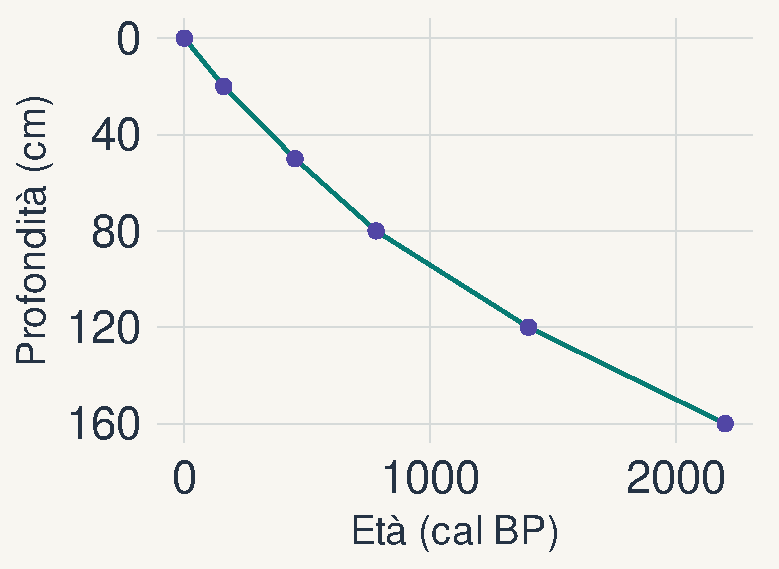
\includegraphics[width=\linewidth,height=6.15cm,keepaspectratio]{Figure/F01.pdf}\par}
\PSmall{Ancore sintetiche in viola e interpolazione lineare a tratti in verde.}
}};
\node[anchor=north west,inner sep=0] at([xshift=10.85cm,yshift=-2.12cm]current page.north west){\Colonna{8.16cm}{\PBody{Il grafico dispone la profondità crescente verso il basso e l’età crescente verso destra, seguendo la convenzione della sezione sedimentaria. I segmenti uniscono esattamente le sei ancore, rendendo riconoscibili i cambiamenti del tasso fra intervalli. La continuità della linea corrisponde a un’assunzione di deposizione senza salti temporali nel modello adottato. Una buona corrispondenza alle ancore è garantita dalla costruzione e non costituisce una verifica indipendente della linearità interna o dell’assenza di lacune sedimentarie.}
}};
\end{tikzpicture}\end{frame}

\begin{frame}[plain]\hypertarget{slide9}{}
\bookmark[level=0,page=9]{Scenari di incertezza cronologica}
\bookmark[level=1,page=9]{Le perturbazioni mantengono l’identità delle ancore}
\begin{tikzpicture}[remember picture,overlay]
\PilotChrome{{\fontsize{15.3}{19}\selectfont Le perturbazioni mantengono l’identità delle ancore}}{SCENARI DI INCERTEZZA CRONOLOGICA}{9}{La distribuzione degli scenari dipende dalle ipotesi sulle ancore e dall’eventuale condizionamento all’ordine.}
\node[anchor=north west,inner sep=0] at([xshift=.96cm,yshift=-2.12cm]current page.north west){\Colonna{9.40cm}{\PBody{Ogni scenario perturba le sei età attraverso variabili normali standard, moltiplicate per le deviazioni standard dichiarate. La prima ancora rimane fissa, poiché la sua deviazione è nulla. Le estrazioni provengono da una tabella comune conservata nei dati, così che il risultato possa essere ricostruito senza dipendere soltanto dal seme di un generatore. L’indipendenza delle perturbazioni e la forma normale sono ipotesi dell’esercizio; distribuzioni calibrate o errori condivisi richiederebbero una costruzione differente.}
\par\smallskip{\centering\adjustbox{max width=.98\linewidth}{$\displaystyle t_j^{(b)}=t_j+\sigma_jZ_j^{(b)},\qquad Z_j^{(b)}\overset{\rm iid}{\sim}N(0{,}1)$}\par\smallskip}
}};
\node[anchor=north west,inner sep=0] at([xshift=10.85cm,yshift=-2.12cm]current page.north west){\Colonna{8.16cm}{\PInfo{j: ancora; b: scenario; $t_j$: età di base; $\sigma_j$: deviazione standard in anni. L’indipendenza vale prima del controllo di monotonicità. Le sequenze non crescenti sono scartate conservando l’identificativo; le età restano associate alle proprie profondità. Gli scenari accettati rappresentano la proposta condizionata all’ordine cronologico.}
}};
\end{tikzpicture}\end{frame}

\begin{frame}[plain]\hypertarget{slide10}{}
\bookmark[level=1,page=10]{L’accettazione resta un risultato verificabile}
\begin{tikzpicture}[remember picture,overlay]
\PilotChrome{L’accettazione resta un risultato verificabile}{SCENARI DI INCERTEZZA CRONOLOGICA}{10}{Numero di scenari generati, accettati e scartati devono essere riportati insieme al criterio di ammissibilità.}
\node[anchor=north west,inner sep=0] at([xshift=.96cm,yshift=-2.12cm]current page.north west){\Colonna{9.40cm}{\PBody{Nel piano utilizzato tutti i cinquecento scenari rispettano l’ordine crescente delle età, per cui nessuna estrazione viene eliminata. Questo esito riguarda le deviazioni standard e i numeri casuali effettivamente adottati; non dimostra che ogni possibile proposta normale sarebbe monotona. Il codice conserva la matrice delle ancore simulate e l’indicatore di accettazione. La tracciabilità consente di ricostruire la curva associata a ciascuna riga e di controllare il rapporto fra distribuzione proposta e distribuzione utilizzata.}
}};
\node[anchor=north west,inner sep=0] at([xshift=10.85cm,yshift=-2.12cm]current page.north west){\Colonna{8.16cm}{\begin{tcolorbox}[enhanced,arc=1.7mm,boxrule=.6pt,colback=white,colframe=Classical!60!Navy,colbacktitle=Navy,coltitle=white,fonttitle=\bfseries\small,title={R · calcolo riproducibile},left=1.7mm,right=1.3mm,top=1.1mm,bottom=1.1mm,before skip=1mm,after skip=1.0mm]\lstinputlisting[style=GeoR,language=R,basicstyle=\ttfamily\fontsize{8.6}{11.4}\selectfont]{Codice/scenari.R}\end{tcolorbox}
\PLabel{Risultato in R}
\begin{tcolorbox}[colback=GeoTint,colframe=Rule,boxrule=.5pt,arc=1.4mm,left=2mm,right=1mm,top=1mm,bottom=1mm]{\fontsize{8.4}{10.9}\selectfont\ttfamily \mbox{\ \ \ \ 2.5\%\ \ \ \ \ \ 50\%\ \ \ \ 97.5\%\ }\\\mbox{2014.427\ 2200.941\ 2391.812\ }}\end{tcolorbox}
}};
\end{tikzpicture}\end{frame}

\begin{frame}[plain]\hypertarget{slide11}{}
\bookmark[level=1,page=11]{La fascia riassume quantili a profondità fissata}
\begin{tikzpicture}[remember picture,overlay]
\PilotChrome{La fascia riassume quantili a profondità fissata}{SCENARI DI INCERTEZZA CRONOLOGICA}{11}{Una fascia di quantili puntuali e una regione simultanea rispondono a domande probabilistiche diverse.}
\node[anchor=north west,inner sep=0] at([xshift=.96cm,yshift=-2.12cm]current page.north west){\Colonna{9.40cm}{{\centering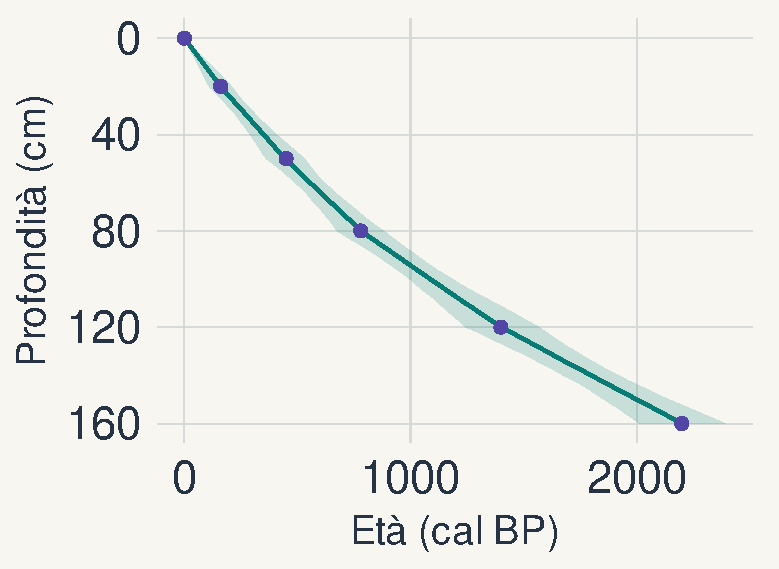
\includegraphics[width=\linewidth,height=6.15cm,keepaspectratio]{Figure/F02.pdf}\par}
\PSmall{Quantili puntuali degli scenari cronologici; profondità fissata.}
}};
\node[anchor=north west,inner sep=0] at([xshift=10.85cm,yshift=-2.12cm]current page.north west){\Colonna{8.16cm}{\PBody{Per ogni profondità della griglia si calcolano i quantili 2,5\%, 50\% e 97,5\% delle età interpolate nei cinquecento scenari. La fascia descrive pertanto un’incertezza puntuale condizionata al modello delle ancore, mentre la linea centrale segue la mediana. A cento centimetri i quantili estremi sono circa 997,745 e 1186,507 anni cal BP. La fascia non è una regione simultanea con probabilità del 95\% per l’intera curva, né include automaticamente errori di profondità, hiatus o scelta del modello deposizionale.}
}};
\end{tikzpicture}\end{frame}

\begin{frame}[plain]\hypertarget{slide12}{}
\bookmark[level=1,page=12]{La verifica analitica della propagazione}
\begin{tikzpicture}[remember picture,overlay]
\PilotChrome{La verifica analitica della propagazione}{SCENARI DI INCERTEZZA CRONOLOGICA}{12}{La simulazione diventa più controllabile quando un caso lineare ammette una verifica analitica.}
\node[anchor=north west,inner sep=0] at([xshift=.96cm,yshift=-2.12cm]current page.north west){\Colonna{9.40cm}{{\centering\resizebox{0.90\linewidth}{!}{\begin{tikzpicture}[x=1cm,y=-.87cm,every node/.style={font=\fontsize{12.2}{15}\selectfont,text=Ink},arr/.style={-{Stealth[length=2mm]},line width=.8pt,draw=Classical}]\path[use as bounding box] (0,0) rectangle (7.45,6.2);
\draw[draw=Classical,fill=Classical!8,rounded corners=2pt,line width=.7pt] (0.7,1) rectangle (3.2,2.5);
\node[anchor=center,text=Ink,font=\fontsize{12}{15}\selectfont,text width=2.3cm,align=center] at (1.95,1.75) {$t_{80},\ \sigma=55$};
\draw[draw=Quantum,fill=Quantum!8,rounded corners=2pt,line width=.7pt] (4.1,1) rectangle (6.6,2.5);
\node[anchor=center,text=Ink,font=\fontsize{12}{15}\selectfont,text width=2.3cm,align=center] at (5.35,1.75) {$t_{120},\ \sigma=80$};
\draw[arr,draw=Classical] (2,2.8)--(3.2,3.7);
\draw[arr,draw=Quantum] (5.3,2.8)--(4.2,3.7);
\node[anchor=center,text=Ink,font=\fontsize{15}{15}\selectfont,text width=6cm,align=center] at (3.7,4.5) {$t_{100}=\frac12t_{80}+\frac12t_{120}$};
\node[anchor=center,text=Ink,font=\fontsize{11}{15}\selectfont,text width=6.8cm,align=center] at (3.7,6) {La covarianza entra nella varianza della somma.};

\end{tikzpicture}}\par}
\PSmall{$\mathbf w$: sei pesi d’interpolazione; $\Sigma$: covarianza delle età, in anni². A 100 cm i due pesi non nulli valgono 1/2.}
}};
\node[anchor=north west,inner sep=0] at([xshift=10.85cm,yshift=-2.12cm]current page.north west){\Colonna{8.16cm}{\PBody{Prima del condizionamento di monotonicità, l’età interpolata è una combinazione lineare delle ancore casuali. La sua varianza si ricava quindi dai pesi e dalla matrice di covarianza. A cento centimetri intervengono, con peso un mezzo, le ancore di ottanta e centoventi centimetri; assumendole indipendenti, la deviazione standard teorica è circa 48,54 anni. Il confronto analitico chiarisce anche il contributo di eventuali errori correlati fra le ancore.}
\par\smallskip{\centering\adjustbox{max width=.98\linewidth}{$\displaystyle \begin{gathered}\operatorname{Var}\{t(z)\}=\mathbf w^T\Sigma\mathbf w\\\operatorname{Var}\{t(100)\}=\frac{55^2+80^2}{4}\end{gathered}$}\par\smallskip}
}};
\end{tikzpicture}\end{frame}

\begin{frame}[plain]\hypertarget{slide13}{}
\bookmark[level=0,page=13]{Massimo osservato e interpretazione temporale}
\bookmark[level=1,page=13]{Il massimo si trova al bordo della sequenza}
\begin{tikzpicture}[remember picture,overlay]
\PilotChrome{Il massimo si trova al bordo della sequenza}{MASSIMO OSSERVATO E INTERPRETAZIONE TEMPORALE}{13}{Un massimo al bordo richiede una conclusione limitata alla porzione effettivamente osservata.}
\node[anchor=north west,inner sep=0] at([xshift=.96cm,yshift=-2.12cm]current page.north west){\Colonna{9.40cm}{{\centering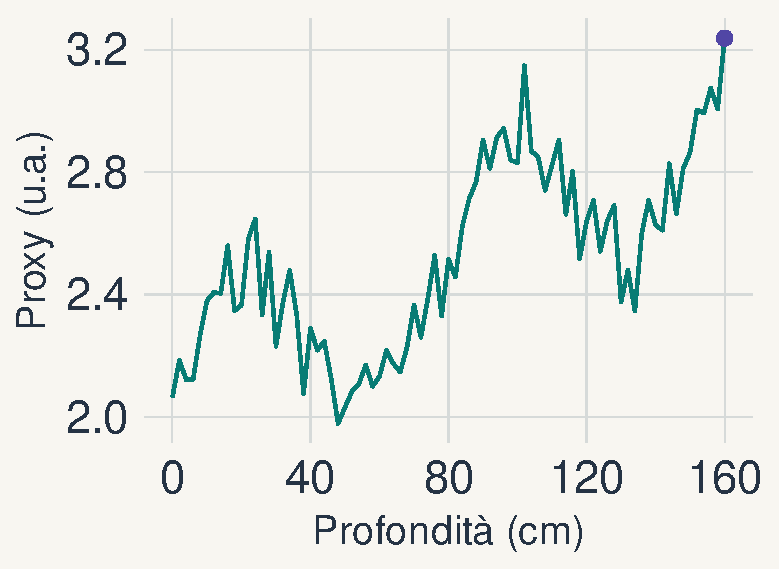
\includegraphics[width=\linewidth,height=6.15cm,keepaspectratio]{Figure/F03.pdf}\par}
\PSmall{Massimo osservato a 160 cm, coincidente con il limite del dominio.}
}};
\node[anchor=north west,inner sep=0] at([xshift=10.85cm,yshift=-2.12cm]current page.north west){\Colonna{8.16cm}{\PBody{Il proxy è misurato ogni due centimetri, da zero a centosessanta. Il valore più elevato del campione si trova nell’ultima posizione, che viene evidenziata in viola. Poiché mancano osservazioni a profondità maggiori, il grafico non documenta una successiva diminuzione e non permette di riconoscere un massimo interno completo. La posizione viene mantenuta fissa nel calcolo cronologico successivo, per cui l’incertezza simulata riguarda l’età assegnata a questo valore osservato, lasciando esclusi errore del proxy e selezione del massimo.}
}};
\end{tikzpicture}\end{frame}

\begin{frame}[plain]\hypertarget{slide14}{}
\bookmark[level=1,page=14]{L’età del massimo segue l’ultima ancora}
\begin{tikzpicture}[remember picture,overlay]
\PilotChrome{L’età del massimo segue l’ultima ancora}{MASSIMO OSSERVATO E INTERPRETAZIONE TEMPORALE}{14}{La distribuzione dell’età condizionata al massimo osservato non esaurisce l’incertezza sulla storia del proxy.}
\node[anchor=north west,inner sep=0] at([xshift=.96cm,yshift=-2.12cm]current page.north west){\Colonna{9.40cm}{{\centering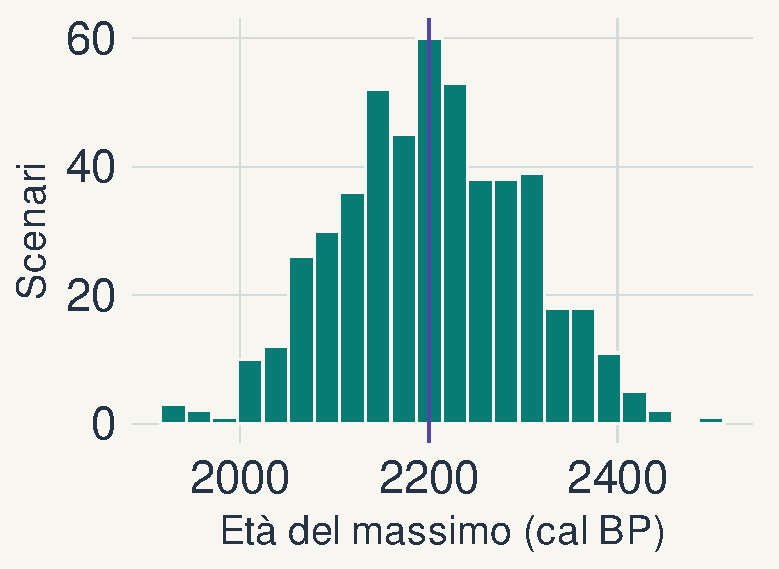
\includegraphics[width=\linewidth,height=6.15cm,keepaspectratio]{Figure/F05.pdf}\par}
\PSmall{$p(z_j)$: proxy alla profondità campionata j, fra 81 misure; $t^*$: cronologia di uno scenario. Massimo fisso a 160 cm; 500 età simulate.}
}};
\node[anchor=north west,inner sep=0] at([xshift=10.85cm,yshift=-2.12cm]current page.north west){\Colonna{8.16cm}{\PBody{Nel modello continuo l’età del massimo osservato è 2200 anni cal BP, perché la profondità corrisponde esattamente all’ultima ancora. In ogni scenario la stessa posizione assume l’età perturbata di quell’ancora, senza contributi di interpolazione da profondità adiacenti. L’istogramma rappresenta questa distribuzione condizionata alla posizione scelta e all’ammissibilità cronologica. La precisione del risultato non misura quanto sia ben localizzato un evento nel processo sedimentario, poiché il campionamento del proxy e l’estensione della sequenza restano fissati.}
\par\smallskip{\centering\adjustbox{max width=.98\linewidth}{$\displaystyle j^*=\arg\max_j p(z_j),\qquad t^*_{max}=t^*(z_{j^*})$}\par\smallskip}
}};
\end{tikzpicture}\end{frame}

\begin{frame}[plain]\hypertarget{slide15}{}
\bookmark[level=1,page=15]{La trasformazione temporale modifica le distanze}
\begin{tikzpicture}[remember picture,overlay]
\PilotChrome{La trasformazione temporale modifica le distanze}{MASSIMO OSSERVATO E INTERPRETAZIONE TEMPORALE}{15}{La cronologia modifica la distanza temporale fra osservazioni, mantenendo invariata la misura del proxy.}
\node[anchor=north west,inner sep=0] at([xshift=.96cm,yshift=-2.12cm]current page.north west){\Colonna{9.40cm}{{\centering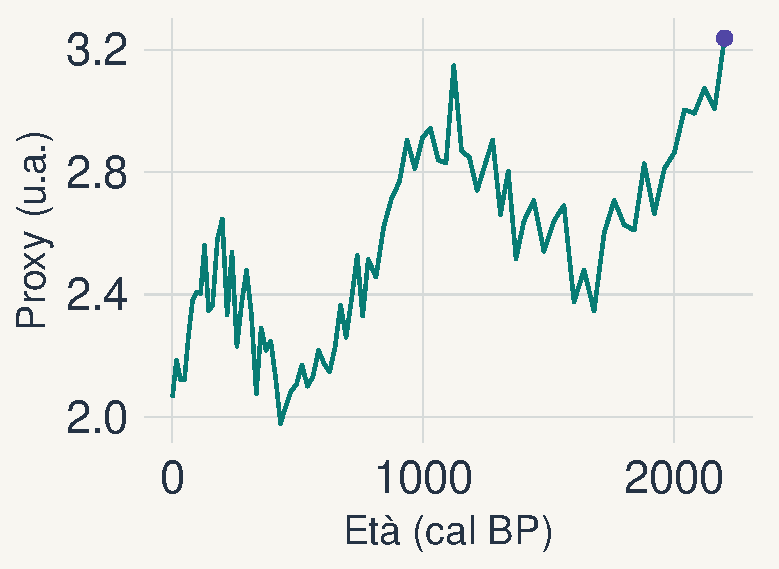
\includegraphics[width=\linewidth,height=6.15cm,keepaspectratio]{Figure/F04.pdf}\par}
\PSmall{Gli stessi valori del proxy nella cronologia continua di riferimento.}
}};
\node[anchor=north west,inner sep=0] at([xshift=10.85cm,yshift=-2.12cm]current page.north west){\Colonna{8.16cm}{\PBody{Applicando la curva cronologica a tutte le profondità, il proxy viene rappresentato in funzione dell’età. I valori misurati rimangono identici, mentre gli intervalli fra osservazioni cambiano secondo il tasso di accumulo dei diversi tratti. La forma visiva della curva dipende quindi anche dalla trasformazione dell’asse orizzontale. Un confronto con altri archivi dovrebbe considerare le rispettive cronologie e incertezze, poiché l’allineamento di due massimi apparenti potrebbe essere alterato dalle ipotesi temporali adottate.}
}};
\end{tikzpicture}\end{frame}

\begin{frame}[plain]\hypertarget{slide16}{}
\bookmark[level=1,page=16]{Passo spaziale costante e tempo irregolare}
\begin{tikzpicture}[remember picture,overlay]
\PilotChrome{Passo spaziale costante e tempo irregolare}{MASSIMO OSSERVATO E INTERPRETAZIONE TEMPORALE}{16}{La risoluzione temporale deriva congiuntamente dal passo di campionamento e dal modello età–profondità.}
\node[anchor=north west,inner sep=0] at([xshift=.96cm,yshift=-2.12cm]current page.north west){\Colonna{9.40cm}{{\centering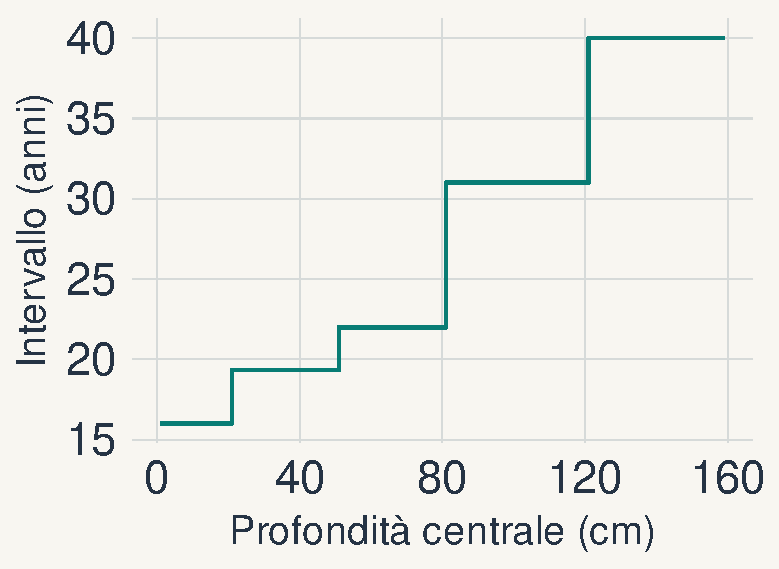
\includegraphics[width=\linewidth,height=6.15cm,keepaspectratio]{Figure/F08.pdf}\par}
\PSmall{Anni intercorrenti fra due campioni distanti 2 cm.}
}};
\node[anchor=north west,inner sep=0] at([xshift=10.85cm,yshift=-2.12cm]current page.north west){\Colonna{8.16cm}{\PBody{Il campionamento ogni due centimetri corrisponde a intervalli temporali che variano da sedici a quaranta anni. Il grafico segue tali distanze lungo la sequenza, mostrando salti quando cambia il tratto cronologico. Una procedura che richieda tempi equidistanti dovrebbe quindi dichiarare una griglia temporale e una regola di interpolazione ulteriore. Aumentare il numero dei punti interpolati renderebbe più densa la rappresentazione numerica, senza aggiungere osservazioni indipendenti né migliorare automaticamente la risoluzione effettiva dell’archivio.}
}};
\end{tikzpicture}\end{frame}

\begin{frame}[plain]\hypertarget{slide17}{}
\bookmark[level=0,page=17]{Hiatus e conclusione condizionata}
\bookmark[level=1,page=17]{Uno hiatus introduce una discontinuità}
\begin{tikzpicture}[remember picture,overlay]
\PilotChrome{Uno hiatus introduce una discontinuità}{HIATUS E CONCLUSIONE CONDIZIONATA}{17}{Un cambiamento strutturale del modello deve restare distinto dalla perturbazione delle età entro lo stesso modello.}
\node[anchor=north west,inner sep=0] at([xshift=.96cm,yshift=-2.12cm]current page.north west){\Colonna{9.40cm}{{\centering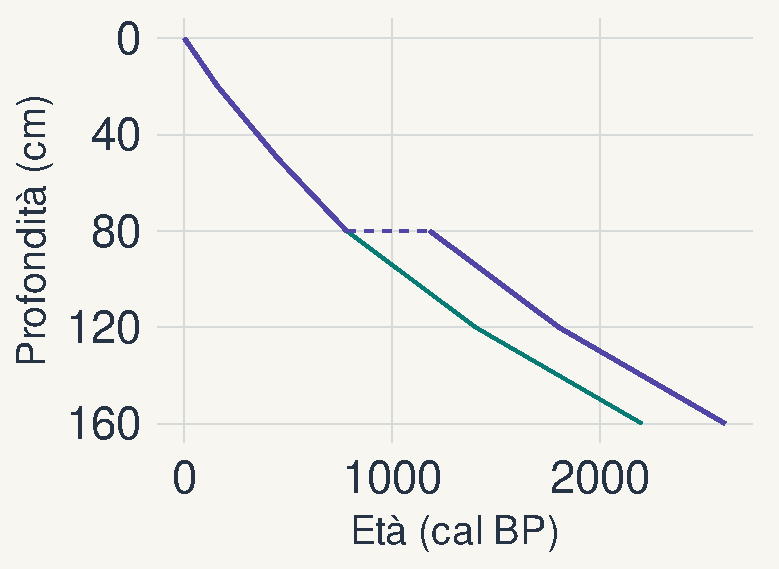
\includegraphics[width=\linewidth,height=6.15cm,keepaspectratio]{Figure/F06.pdf}\par}
\PSmall{z: profondità in cm; t(z): età continua in anni cal BP. $t_H$: scenario con 400 anni aggiunti per z > 80 cm.}
}};
\node[anchor=north west,inner sep=0] at([xshift=10.85cm,yshift=-2.12cm]current page.north west){\Colonna{8.16cm}{\PBody{La sensibilità aggiunge quattrocento anni alle età sotto ottanta centimetri, lasciando invariata la parte superiore. La curva presenta così due rami separati alla stessa profondità, che rappresentano un intervallo temporale privo di deposizione nel modello. Il salto viene mostrato esplicitamente, evitando di collegarlo con un segmento obliquo che suggerirebbe accumulo continuo. Questa costruzione modifica anche le ancore inferiori e costituisce uno scenario alternativo dichiarato; non è un’evidenza di hiatus ricavata dalle sei età originarie.}
\par\smallskip{\centering\adjustbox{max width=.98\linewidth}{$\displaystyle t_H(z)=t(z)+400\,\mathbf1\{z>80\}$}\par\smallskip}
}};
\end{tikzpicture}\end{frame}

\begin{frame}[plain]\hypertarget{slide18}{}
\bookmark[level=1,page=18]{Lo scenario sposta l’età attribuita al massimo}
\begin{tikzpicture}[remember picture,overlay]
\PilotChrome{Lo scenario sposta l’età attribuita al massimo}{HIATUS E CONCLUSIONE CONDIZIONATA}{18}{Incertezza entro un modello e sensibilità alla sua struttura richiedono due resoconti distinti.}
\node[anchor=north west,inner sep=0] at([xshift=.96cm,yshift=-2.12cm]current page.north west){\Colonna{9.40cm}{{\centering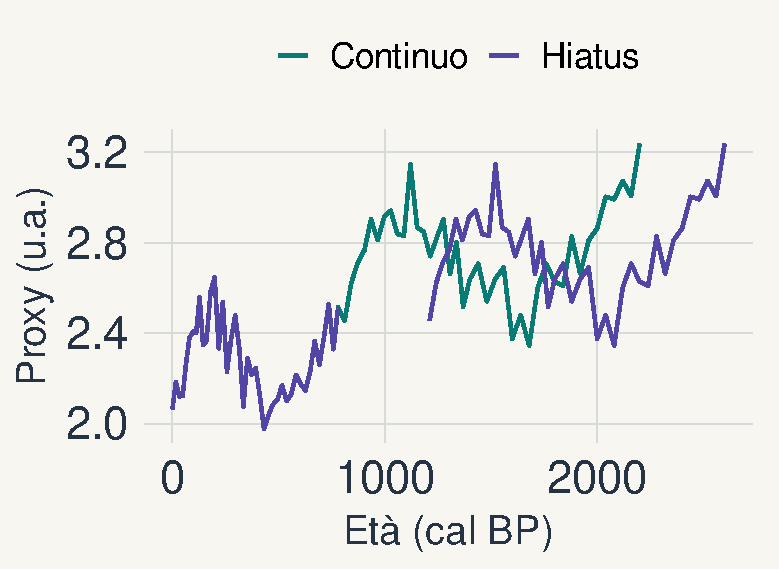
\includegraphics[width=\linewidth,height=6.15cm,keepaspectratio]{Figure/F07.pdf}\par}
\PSmall{Confronto delle cronologie; nel modello con hiatus il salto resta aperto.}
}};
\node[anchor=north west,inner sep=0] at([xshift=10.85cm,yshift=-2.12cm]current page.north west){\Colonna{8.16cm}{\PBody{Con lo hiatus ipotizzato, il massimo a centosessanta centimetri passa da 2200 a 2600 anni cal BP. La figura confronta il proxy nelle due cronologie, interrompendo la curva alternativa attraverso il salto temporale. La differenza di quattrocento anni descrive una sensibilità strutturale determinata dall’ipotesi aggiunta, che non viene incorporata nei quantili degli scenari normali. Una conclusione completa presenta separatamente la stima nel modello continuo, la sua incertezza condizionata e il cambiamento prodotto dal modello con lacuna.}
}};
\end{tikzpicture}\end{frame}

\begin{frame}[plain]\hypertarget{slide19}{}
\bookmark[level=1,page=19]{Consegna: delimitare l’interpretazione del massimo}
\begin{tikzpicture}[remember picture,overlay]
\PilotChrome{Consegna: delimitare l’interpretazione del massimo}{HIATUS E CONCLUSIONE CONDIZIONATA}{19}{L’interpretazione geologica rimane proporzionata al dominio osservato e alle ipotesi della cronologia.}
\node[anchor=north west,inner sep=0] at([xshift=.96cm,yshift=-2.12cm]current page.north west){\Colonna{9.40cm}{\PBody{La relazione presenta audit delle ancore, curva continua, propagazione delle età, posizione del massimo e confronto con lo hiatus. L’esercizio richiede di ricavare l’età a trentacinque centimetri e la varianza a cento, spiegando quali assunzioni intervengano nei due calcoli. La discussione finale chiarisce perché il massimo al bordo non dimostri un evento culminato entro la sequenza e quali nuove osservazioni potrebbero sostenerne una ricostruzione più ampia. La conclusione distingue esplicitamente dati sintetici, modello cronologico e bersaglio temporale.}
}};
\node[anchor=north west,inner sep=0] at([xshift=10.85cm,yshift=-2.12cm]current page.north west){\Colonna{8.16cm}{\PInfo{R/P08\_figure.R riunisce audit, interpolazione, scenari e attribuzione dell’età al massimo, conservando ancore simulate e quantili. I laboratori M13 sviluppano separatamente i calcoli che il progetto collega in un’unica argomentazione cronologica.}
}};
\end{tikzpicture}\end{frame}

\begin{frame}[plain]\hypertarget{slide20}{}
\bookmark[level=0,page=20]{Laboratori della spedizione}
\bookmark[level=1,page=20]{Tre fasi della spedizione nel laboratorio}
\begin{tikzpicture}[remember picture,overlay]
\PilotChrome{Tre fasi della spedizione nel laboratorio}{LABORATORI DELLA SPEDIZIONE}{20}{Gli esperimenti usano sequenze sintetiche; la conclusione sul caso resta quella ottenuta dalle sei ancore.}
\node[anchor=north west,inner sep=0] at([xshift=.96cm,yshift=-2.12cm]current page.north west){\Colonna{9.40cm}{{\centering\resizebox{0.97\linewidth}{!}{\begin{tikzpicture}[x=1cm,y=1cm,every node/.style={font=\sffamily\fontsize{9.2}{11}\selectfont,text=Ink}]
\node[draw=Classical,fill=Classical,rounded corners=2mm,text=white,text width=2.45cm,align=flush center,minimum height=1.55cm,anchor=west,font=\sffamily\bfseries\fontsize{9.2}{11}\selectfont] (f0) at (0,0.00) {1. Stabilire le ancore};
\node[draw=Classical!60,fill=Classical!6,rounded corners=1.5mm,line width=.6pt,text width=2.8cm,align=flush center,minimum height=1.55cm,anchor=west] (e00) at (2.95,0.00) {Ancore cronologiche e convenzioni temporali\\[1pt]{\fontsize{7.6}{9}\selectfont\color{Muted}m13-ancore}};
\node[draw=Rule,fill=white,rounded corners=1.5mm,line width=.6pt,text width=2.8cm,align=flush center,minimum height=1.55cm,anchor=west] (e01) at (6.10,0.00) {Interpolazione e tassi di accumulo\\[1pt]{\fontsize{7.6}{9}\selectfont\color{Muted}m13-interpolazione}};
\draw[pEdge] (f0.east)--(e00.west);
\node[draw=Classical,fill=Classical,rounded corners=2mm,text=white,text width=2.45cm,align=flush center,minimum height=1.55cm,anchor=west,font=\sffamily\bfseries\fontsize{9.2}{11}\selectfont] (f1) at (0,-1.95) {2. Propagare l’incertezza};
\draw[pEdge] (f0.south)--(f1.north);
\node[draw=Classical!60,fill=Classical!6,rounded corners=1.5mm,line width=.6pt,text width=2.8cm,align=flush center,minimum height=1.55cm,anchor=west] (e10) at (2.95,-1.95) {Scenari cronologici e propagazione\\[1pt]{\fontsize{7.6}{9}\selectfont\color{Muted}m13-incertezza}};
\node[draw=Rule,fill=white,rounded corners=1.5mm,line width=.6pt,text width=2.8cm,align=flush center,minimum height=1.55cm,anchor=west] (e11) at (6.10,-1.95) {Durate entro uno stesso scenario\\[1pt]{\fontsize{7.6}{9}\selectfont\color{Muted}m13-durate}};
\draw[pEdge] (f1.east)--(e10.west);
\node[draw=Classical,fill=Classical,rounded corners=2mm,text=white,text width=2.45cm,align=flush center,minimum height=1.55cm,anchor=west,font=\sffamily\bfseries\fontsize{9.2}{11}\selectfont] (f2) at (0,-3.90) {3. Valutare interpretazioni alternative};
\draw[pEdge] (f1.south)--(f2.north);
\node[draw=Classical!60,fill=Classical!6,rounded corners=1.5mm,line width=.6pt,text width=2.8cm,align=flush center,minimum height=1.55cm,anchor=west] (e20) at (2.95,-3.90) {Risoluzione temporale di un proxy\\[1pt]{\fontsize{7.6}{9}\selectfont\color{Muted}m13-proxy}};
\node[draw=Rule,fill=white,rounded corners=1.5mm,line width=.6pt,text width=2.8cm,align=flush center,minimum height=1.55cm,anchor=west] (e21) at (6.10,-3.90) {Discontinuità e sensibilità della cronologia\\[1pt]{\fontsize{7.6}{9}\selectfont\color{Muted}m13-hiatus}};
\draw[pEdge] (f2.east)--(e20.west);
\end{tikzpicture}
}\par}
\PSmall{Fasi della spedizione. Il primo esperimento di ogni fase ha le pagine Scenario A e Confronto.}
}};
\node[anchor=north west,inner sep=0] at([xshift=10.85cm,yshift=-2.12cm]current page.north west){\Colonna{8.16cm}{\PBody{Gli esperimenti della lezione Strata ripetono su sequenze sintetiche tre passaggi della spedizione: stabilire le ancore, propagare l’incertezza delle età, confrontare interpretazioni alternative del proxy. Ogni fase ha uno scenario di partenza e un confronto con un solo parametro modificato.}
\vspace{.2cm}\PLabel{Altri esperimenti delle fasi}
\PLab{https://marzione00.github.io/Lab_Geo/\#laboratorio/m13-interpolazione}{Interpolazione e tassi di accumulo · m13-interpolazione}
\PLab{https://marzione00.github.io/Lab_Geo/\#laboratorio/m13-durate}{Durate entro uno stesso scenario · m13-durate}
\PLab{https://marzione00.github.io/Lab_Geo/\#laboratorio/m13-hiatus}{Discontinuità e sensibilità della cronologia · m13-hiatus}
}};
\end{tikzpicture}\end{frame}

\begin{frame}[plain]\hypertarget{slide21}{}
\bookmark[level=1,page=21]{Ancore cronologiche e convenzioni temporali}
\begin{tikzpicture}[remember picture,overlay]
\PilotChrome{Ancore cronologiche e convenzioni temporali}{LABORATORI DELLA SPEDIZIONE}{21}{Collegare profondità, età e riferimento temporale.}
\node[anchor=north west,inner sep=0] at([xshift=.96cm,yshift=-2.12cm]current page.north west){\Colonna{9.40cm}{{\centering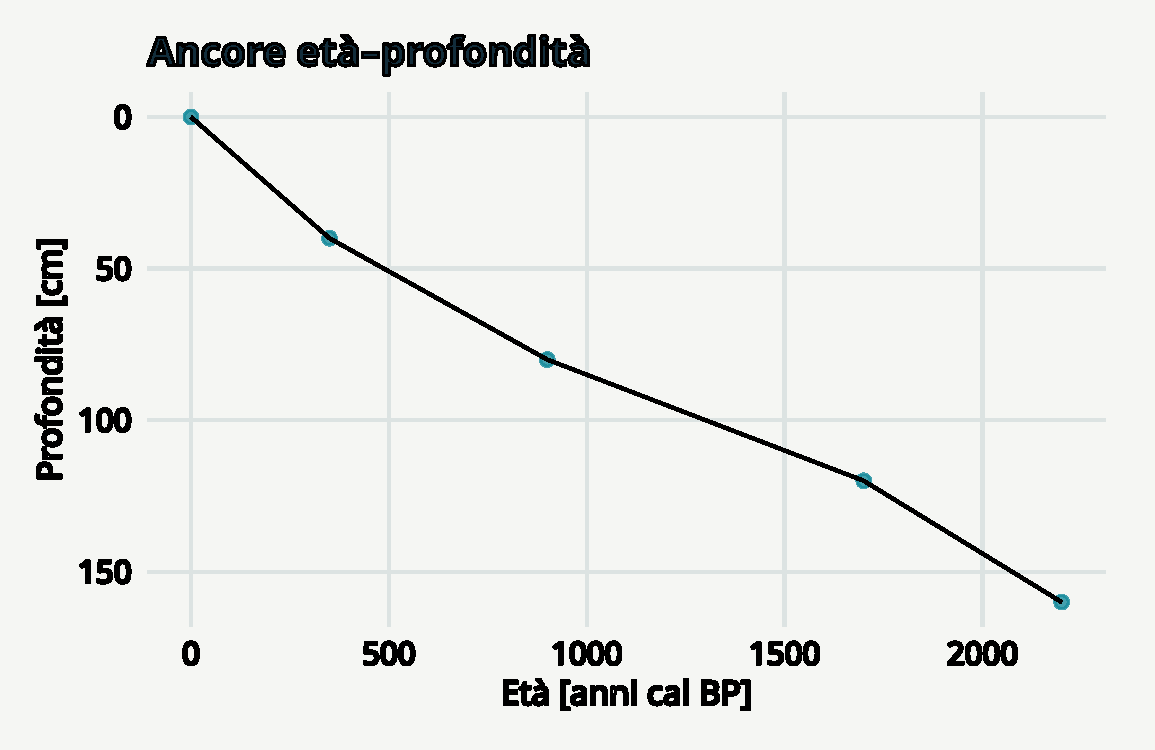
\includegraphics[width=\linewidth,height=6.0cm,keepaspectratio]{Esperimenti/m13-ancore-A.pdf}\par}
\PSmall{Età dell’ancora a 80 cm [anni cal BP]: 900. Seme: 17.}
}};
\node[anchor=north west,inner sep=0] at([xshift=10.85cm,yshift=-2.12cm]current page.north west){\Colonna{8.16cm}{\PLabel{Scenario A · simulazione}
\PBody{Un’ancora cronologica associa una profondità a un’età, mantenendo il legame con il livello stratigrafico dal quale deriva. Le cinque ancore dell’esperimento sono sintetiche e già espresse in anni di calendario BP; il controllo modifica quella situata a ottanta centimetri. La carta mostra come questa scelta cambi la relazione locale fra spessore ed età.}
\par\smallskip{\centering\adjustbox{max width=.98\linewidth}{$\displaystyle a_{astronomico}=1950-t_{cal\,BP}$}\par\smallskip}
\PSmall{$T_{\mathrm{cal\,BP}}$ è l’età di calendario rispetto al 1950; l’anno astronomico si ottiene sottraendo tale età da 1950. Profondità crescenti ed età crescenti definiscono la monotonicità controllata dal programma.}
}};
\node[anchor=north east,inner sep=0] at([xshift=17.1cm,yshift=-12.04cm]current page.north west){\fontsize{7.7}{9}\selectfont \href{https://marzione00.github.io/Lab_Geo/\#laboratorio/m13-ancore}{\color{Classical}\bfseries Apri il laboratorio · m13-ancore}};
\end{tikzpicture}\end{frame}

\begin{frame}[plain]\hypertarget{slide22}{}
\bookmark[level=1,page=22]{Confronto | Ancore cronologiche e convenzioni temporali}
\begin{tikzpicture}[remember picture,overlay]
\PilotChrome{{\fontsize{15.3}{19}\selectfont Confronto | Ancore cronologiche e convenzioni temporali}}{LABORATORI DELLA SPEDIZIONE}{22}{Le ancore associano età e profondità; la convenzione BP usa il 1950 come riferimento.}
\node[anchor=north west,inner sep=0] at([xshift=.96cm,yshift=-2.12cm]current page.north west){\Colonna{9.40cm}{{\centering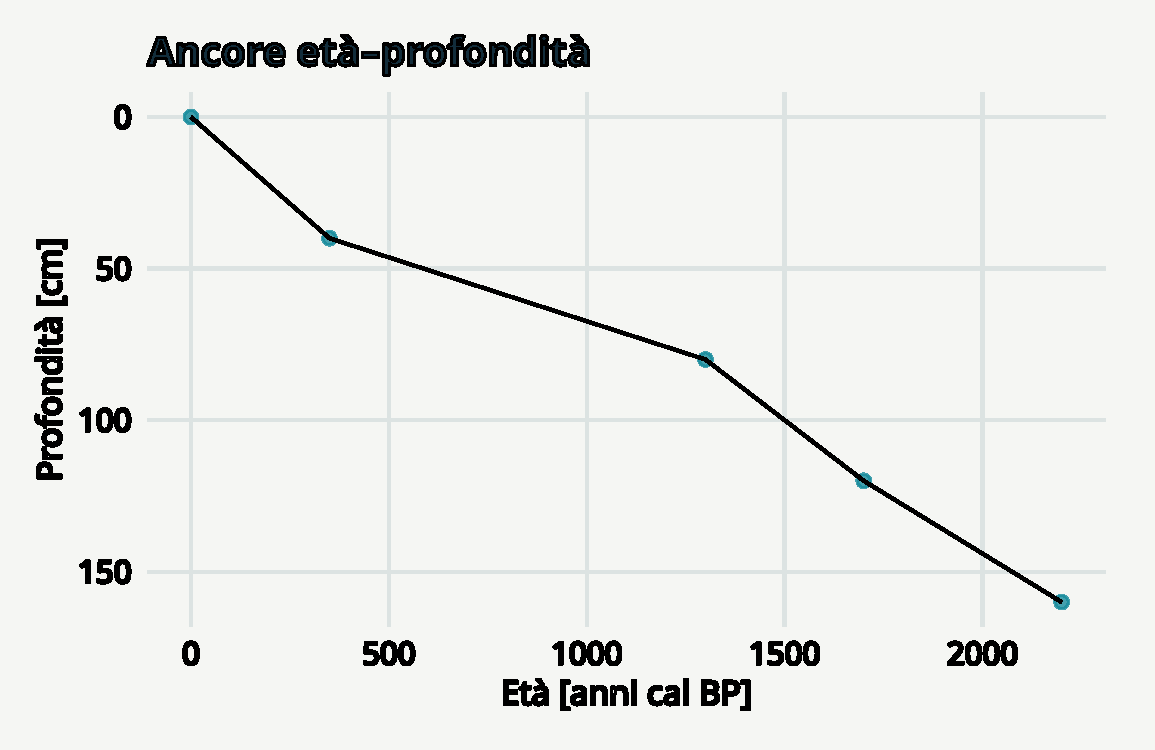
\includegraphics[width=\linewidth,height=5.6cm,keepaspectratio]{Esperimenti/m13-ancore-B.pdf}\par}
\PSmall{Età dell’ancora a 80 cm [anni cal BP]: 900 $\to$ 1300. Tutti gli altri parametri e il seme sono fissi.}
}};
\node[anchor=north west,inner sep=0] at([xshift=10.85cm,yshift=-2.12cm]current page.north west){\Colonna{8.16cm}{\PLabel{Confronto fra gli scenari}
{\fontsize{10.2}{12.8}\selectfont\begin{tabular}{@{}>{\raggedright\arraybackslash}p{0.48\linewidth}@{\hspace{.13cm}}>{\raggedright\arraybackslash}p{0.224\linewidth}@{\hspace{.13cm}}>{\raggedright\arraybackslash}p{0.224\linewidth}@{}}\toprule Grandezza & A & B\\[2.3pt]
\midrule 
Anno astronomico dell’ancora & 1050 & 650\\[2.3pt]
Ancore & 5 & 5\\[2.3pt]
Cronologia monotona & 1 & 1\\[2.3pt]
\bottomrule\end{tabular}\par}
\vspace{.25cm}\PBody{Portando l’ancora da 900 a 1300 anni BP, l’anno astronomico corrispondente passa da 1050 a 650. Le cinque ancore del simulatore conservano l’ordine.}
}};
\node[anchor=north east,inner sep=0] at([xshift=17.1cm,yshift=-12.04cm]current page.north west){\fontsize{7.7}{9}\selectfont \href{https://marzione00.github.io/Lab_Geo/\#laboratorio/m13-ancore}{\color{Classical}\bfseries Apri il laboratorio · m13-ancore}};
\end{tikzpicture}\end{frame}

\begin{frame}[plain]\hypertarget{slide23}{}
\bookmark[level=1,page=23]{Scenari cronologici e propagazione}
\begin{tikzpicture}[remember picture,overlay]
\PilotChrome{Scenari cronologici e propagazione}{LABORATORI DELLA SPEDIZIONE}{23}{Costruire cronologie perturbate conservando l’associazione fra età e profondità.}
\node[anchor=north west,inner sep=0] at([xshift=.96cm,yshift=-2.12cm]current page.north west){\Colonna{9.40cm}{{\centering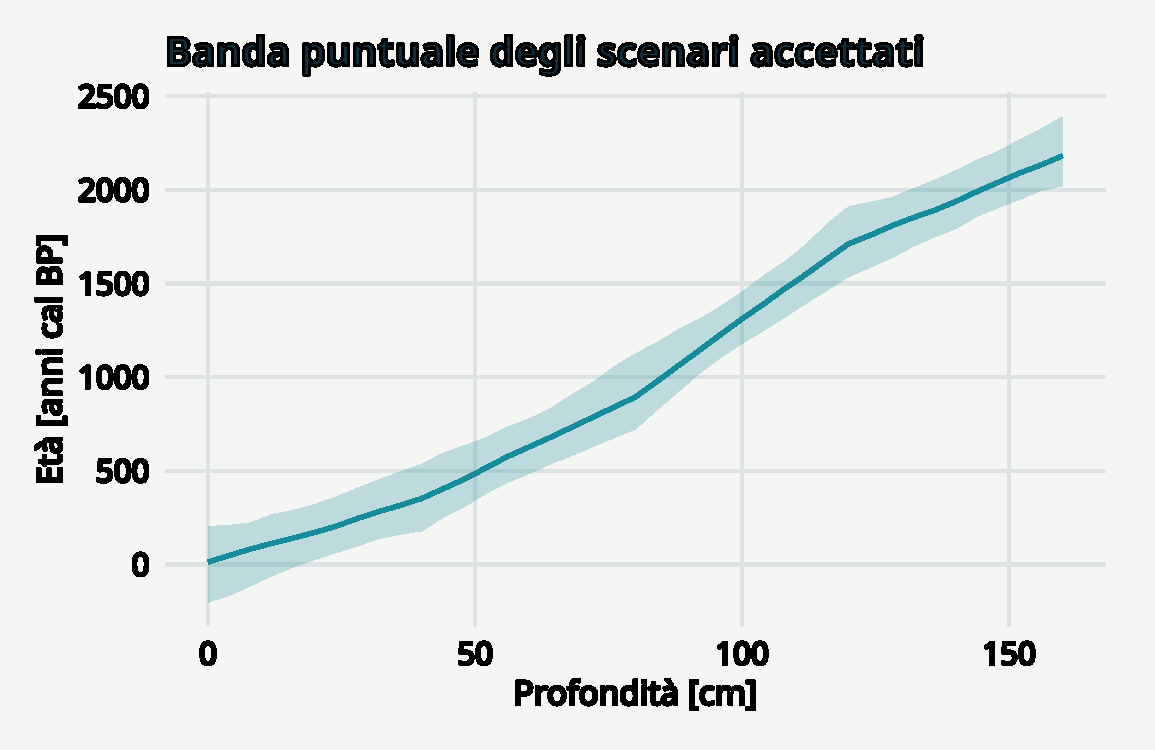
\includegraphics[width=\linewidth,height=6.0cm,keepaspectratio]{Esperimenti/m13-incertezza-A.pdf}\par}
\PSmall{SD delle ancore [anni]: 100. Seme: 17.}
}};
\node[anchor=north west,inner sep=0] at([xshift=10.85cm,yshift=-2.12cm]current page.north west){\Colonna{8.16cm}{\PLabel{Scenario A · simulazione}
\PBody{L’incertezza delle ancore si propaga alle età interpolate perché ciascuna previsione combina le datazioni circostanti. L’esperimento perturba tutte le cinque ancore, compresa quella superficiale, mediante errori gaussiani indipendenti con deviazione standard comune. Ogni configurazione conserva l’associazione fra età e profondità e viene accettata soltanto quando le età rimangono strettamente crescenti.}
\par\smallskip{\centering\adjustbox{max width=.98\linewidth}{$\displaystyle t_b(z)=\operatorname{interp}\{(z_i,t_{i,b})\}$}\par\smallskip}
\PSmall{$z_i$ indica la profondità dell’ancora i e $t_{i,b}$ la sua età nella replica b. $t_b$(z) è la cronologia ottenuta interpolando le ancore della stessa replica; la dispersione controllata è espressa in anni.}
}};
\node[anchor=north east,inner sep=0] at([xshift=17.1cm,yshift=-12.04cm]current page.north west){\fontsize{7.7}{9}\selectfont \href{https://marzione00.github.io/Lab_Geo/\#laboratorio/m13-incertezza}{\color{Classical}\bfseries Apri il laboratorio · m13-incertezza}};
\end{tikzpicture}\end{frame}

\begin{frame}[plain]\hypertarget{slide24}{}
\bookmark[level=1,page=24]{Confronto | Scenari cronologici e propagazione}
\begin{tikzpicture}[remember picture,overlay]
\PilotChrome{Confronto | Scenari cronologici e propagazione}{LABORATORI DELLA SPEDIZIONE}{24}{La selezione degli scenari monotoni condiziona la distribuzione delle cronologie accettate.}
\node[anchor=north west,inner sep=0] at([xshift=.96cm,yshift=-2.12cm]current page.north west){\Colonna{9.40cm}{{\centering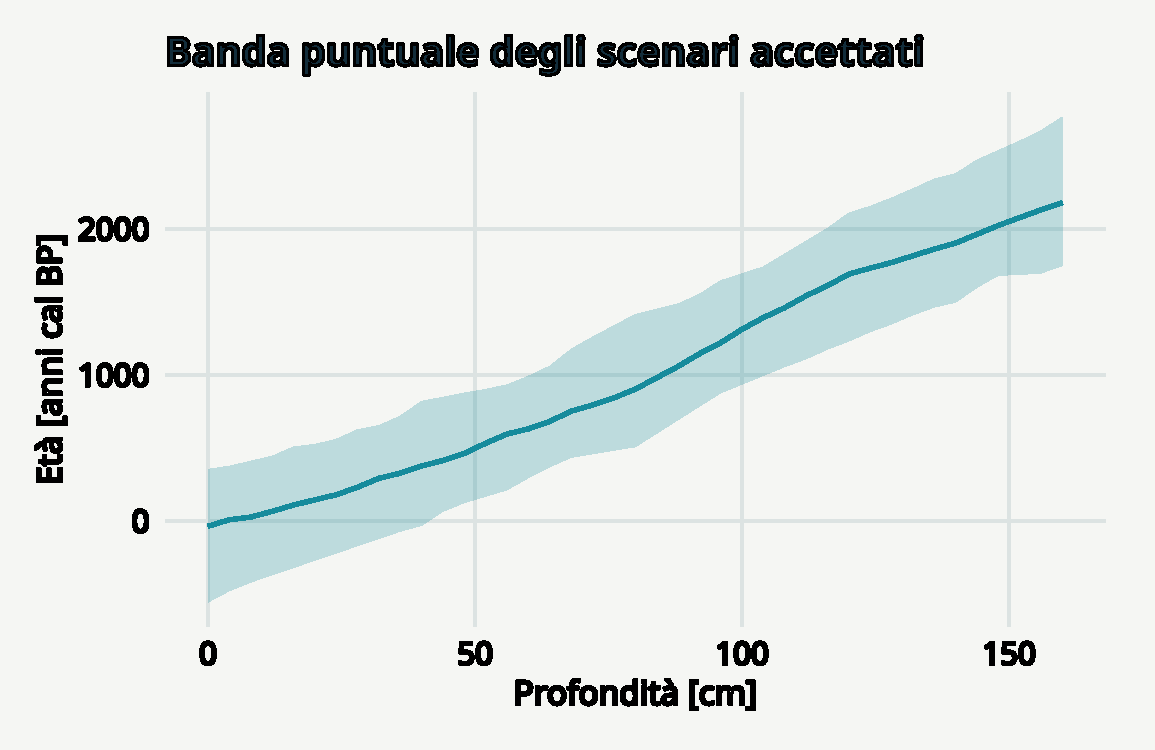
\includegraphics[width=\linewidth,height=5.6cm,keepaspectratio]{Esperimenti/m13-incertezza-B.pdf}\par}
\PSmall{SD delle ancore [anni]: 100 $\to$ 300. Tutti gli altri parametri e il seme sono fissi.}
}};
\node[anchor=north west,inner sep=0] at([xshift=10.85cm,yshift=-2.12cm]current page.north west){\Colonna{8.16cm}{\PLabel{Confronto fra gli scenari}
{\fontsize{10.2}{12.8}\selectfont\begin{tabular}{@{}>{\raggedright\arraybackslash}p{0.48\linewidth}@{\hspace{.13cm}}>{\raggedright\arraybackslash}p{0.224\linewidth}@{\hspace{.13cm}}>{\raggedright\arraybackslash}p{0.224\linewidth}@{}}\toprule Grandezza & A & B\\[2.3pt]
\midrule 
Scenari generati & 200 & 200\\[2.3pt]
Accettati & 199 & 121\\[2.3pt]
Rifiutati & 1 & 79\\[2.3pt]
Ampiezza mediana banda [anni] & 318 & 812\\[2.3pt]
\bottomrule\end{tabular}\par}
\vspace{.25cm}\PBody{Con deviazione standard 300 anni le cronologie accettate scendono a 121 su 200. Anche dopo il controllo di monotonicità le bande si allargano.}
}};
\node[anchor=north east,inner sep=0] at([xshift=17.1cm,yshift=-12.04cm]current page.north west){\fontsize{7.7}{9}\selectfont \href{https://marzione00.github.io/Lab_Geo/\#laboratorio/m13-incertezza}{\color{Classical}\bfseries Apri il laboratorio · m13-incertezza}};
\end{tikzpicture}\end{frame}

\begin{frame}[plain]\hypertarget{slide25}{}
\bookmark[level=1,page=25]{Risoluzione temporale di un proxy}
\begin{tikzpicture}[remember picture,overlay]
\PilotChrome{Risoluzione temporale di un proxy}{LABORATORI DELLA SPEDIZIONE}{25}{Confrontare un campionamento uniforme in profondità con il suo supporto temporale.}
\node[anchor=north west,inner sep=0] at([xshift=.96cm,yshift=-2.12cm]current page.north west){\Colonna{9.40cm}{{\centering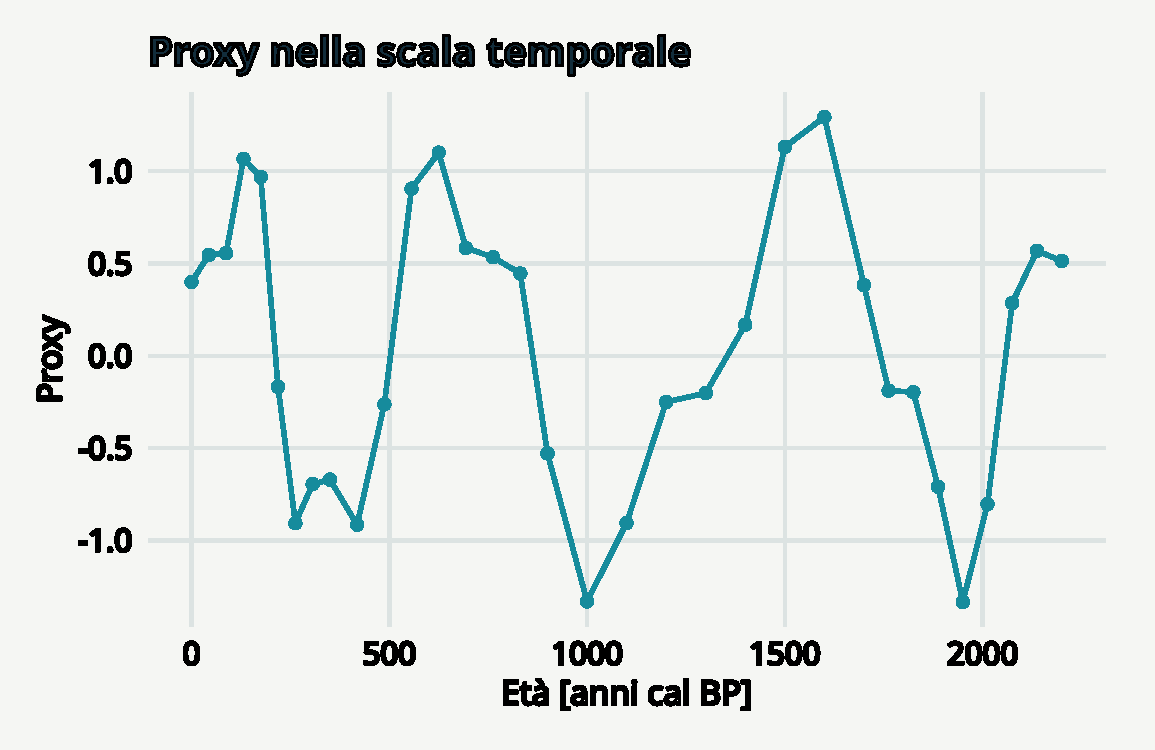
\includegraphics[width=\linewidth,height=6.0cm,keepaspectratio]{Esperimenti/m13-proxy-A.pdf}\par}
\PSmall{Passo in profondità [cm]: 5. Seme: 17.}
}};
\node[anchor=north west,inner sep=0] at([xshift=10.85cm,yshift=-2.12cm]current page.north west){\Colonna{8.16cm}{\PLabel{Scenario A · simulazione}
\PBody{Un campionamento regolare in profondità produce intervalli temporali variabili quando il tasso apparente di accumulo cambia lungo l’archivio. Il proxy sintetico viene osservato a un passo controllabile in centimetri e ciascuna profondità riceve un’età mediante la cronologia a tratti. I punti della figura indicano le osservazioni effettivamente generate, rendendo visibile la loro distribuzione nel tempo.}
\par\smallskip{\centering\adjustbox{max width=.98\linewidth}{$\displaystyle \Delta t_i=t(z_{i+1})-t(z_i)$}\par\smallskip}
\PSmall{$z_i$ e $z_{i+1}$ sono profondità consecutive; t(z) è l’età assegnata dalla cronologia; $\Delta t_i$ è la durata rappresentata dall’intervallo fra i campioni. Il passo in centimetri rimane uniforme, mentre $\Delta t_i$ può variare.}
}};
\node[anchor=north east,inner sep=0] at([xshift=17.1cm,yshift=-12.04cm]current page.north west){\fontsize{7.7}{9}\selectfont \href{https://marzione00.github.io/Lab_Geo/\#laboratorio/m13-proxy}{\color{Classical}\bfseries Apri il laboratorio · m13-proxy}};
\end{tikzpicture}\end{frame}

\begin{frame}[plain]\hypertarget{slide26}{}
\bookmark[level=1,page=26]{Confronto | Risoluzione temporale di un proxy}
\begin{tikzpicture}[remember picture,overlay]
\PilotChrome{Confronto | Risoluzione temporale di un proxy}{LABORATORI DELLA SPEDIZIONE}{26}{Una risoluzione costante in profondità può corrispondere a risoluzioni temporali differenti.}
\node[anchor=north west,inner sep=0] at([xshift=.96cm,yshift=-2.12cm]current page.north west){\Colonna{9.40cm}{{\centering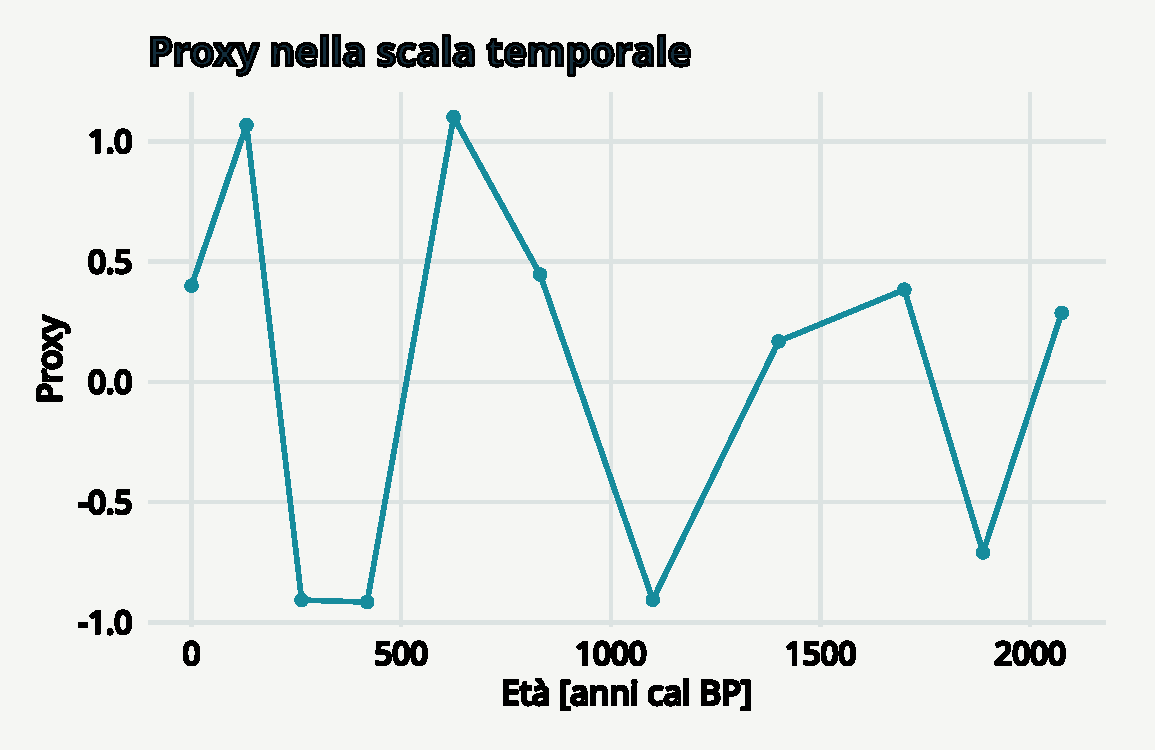
\includegraphics[width=\linewidth,height=5.6cm,keepaspectratio]{Esperimenti/m13-proxy-B.pdf}\par}
\PSmall{Passo in profondità [cm]: 5 $\to$ 15. Tutti gli altri parametri e il seme sono fissi.}
}};
\node[anchor=north west,inner sep=0] at([xshift=10.85cm,yshift=-2.12cm]current page.north west){\Colonna{8.16cm}{\PLabel{Confronto fra gli scenari}
{\fontsize{10.2}{12.8}\selectfont\begin{tabular}{@{}>{\raggedright\arraybackslash}p{0.48\linewidth}@{\hspace{.13cm}}>{\raggedright\arraybackslash}p{0.224\linewidth}@{\hspace{.13cm}}>{\raggedright\arraybackslash}p{0.224\linewidth}@{}}\toprule Grandezza & A & B\\[2.3pt]
\midrule 
Campioni & 33 & 11\\[2.3pt]
Intervallo minimo [anni] & 43,8 & 131\\[2.3pt]
Intervallo massimo [anni] & 100 & 300\\[2.3pt]
\bottomrule\end{tabular}\par}
\vspace{.25cm}\PBody{Il passo triplicato porta da 33 a 11 campioni. La durata massima fra livelli cresce da 100 a 300 anni.}
}};
\node[anchor=north east,inner sep=0] at([xshift=17.1cm,yshift=-12.04cm]current page.north west){\fontsize{7.7}{9}\selectfont \href{https://marzione00.github.io/Lab_Geo/\#laboratorio/m13-proxy}{\color{Classical}\bfseries Apri il laboratorio · m13-proxy}};
\end{tikzpicture}\end{frame}

\begin{frame}[plain]\hypertarget{slide27}{}
\bookmark[level=1,page=27]{Dal risultato alla relazione}
\begin{tikzpicture}[remember picture,overlay]
\PilotChrome{Dal risultato alla relazione}{SINTESI}{27}{Riporta età, unità cal BP, quantili degli scenari e l’effetto dello hiatus come ipotesi distinta.}
\node[anchor=north west,inner sep=0] at([xshift=.96cm,yshift=-2.12cm]current page.north west){\Colonna{9.40cm}{\PLabel{Domanda di partenza}
\PBody{A quale età corrisponde il massimo del proxy, e quanto dipende dalla cronologia adottata?}
\PLabel{Risultato da discutere}
\PBody{Nel modello continuo il massimo, a 160 centimetri, ha un’età di circa 2200 anni cal BP; i quantili 2,5 e 97,5 per cento dei 500 scenari cronologici vanno da circa 2014 a 2392 anni. Con lo hiatus ipotizzato la stessa profondità passa a 2600 anni.}
}};
\node[anchor=north west,inner sep=0] at([xshift=10.85cm,yshift=-2.12cm]current page.north west){\Colonna{8.16cm}{\PLabel{Limiti della conclusione}
\PBody{Il massimo coincide con il bordo inferiore della sequenza e può precedere il culmine di un evento non campionato. La differenza di 400 anni prodotta dallo hiatus è una sensibilità strutturale, separata dai quantili degli scenari continui.}
\vspace{.4cm}\href{https://marzione00.github.io/Lab_Geo/\#modulo-P09}{\color{Classical}\bfseries Prosegui · P09 · Un livello raro e la sua incertezza}
}};
\end{tikzpicture}\end{frame}

\begin{frame}[plain]\hypertarget{slide28}{}
\bookmark[level=1,page=28]{Fonti, dati e codice per riprodurre le figure}
\begin{tikzpicture}[remember picture,overlay]
\PilotChrome{Fonti, dati e codice per riprodurre le figure}{RIFERIMENTI}{28}{I risultati numerici si riferiscono ai dati e alle ipotesi dichiarate nel caso.}
\node[anchor=north west,inner sep=0] at([xshift=.96cm,yshift=-2.12cm]current page.north west){\Colonna{9.40cm}{\PLabel{Dati e attribuzioni}
\PBody{Dati sintetici del corso (proxy\_v3.csv, cronologia\_v3.csv e numeri casuali comuni), con età in anni cal BP secondo la convenzione del radiocarbonio, in raccordo con il modulo M13.}
}};
\node[anchor=north west,inner sep=0] at([xshift=10.85cm,yshift=-2.12cm]current page.north west){\Colonna{8.16cm}{\PLabel{Nell’archivio dei sorgenti}
\PBody{Codice contiene i frammenti delle pagine; R contiene lo script P08\_figure.R, che ricostruisce figure e valori dai dati. Esperimenti comprende i programmi dei due scenari, Diagrammi i disegni TikZ modificabili, Scena il modello Blender della copertina.}
\vspace{.4cm}\href{https://marzione00.github.io/Lab_Geo/\#modulo-P08}{\color{Classical}\bfseries Apri la spedizione P08 su GeoStat Lab}
}};
\end{tikzpicture}\end{frame}
\end{document}
